% Parkinson's Disease Voice Classification - MSc Thesis
% Main document file

\documentclass[11pt,a4paper,oneside,openany]{report}

% All packages, configuration, and custom commands
% Parkinson's Disease Voice Classification - MSc Thesis
% Preamble: All packages, configuration, and custom commands

%% ============================================================================
%% DOCUMENT METADATA
%% ============================================================================

% Author information
\newcommand{\myAuthor}{Μάριος Χρήστος Συρμακέζης}
\newcommand{\myTitle}{Voice-Based Classification of Parkinson's Disease Using Classical Machine Learning}
\newcommand{\myTitleLineBreak}{Voice-Based Classification of Parkinson's Disease Using Classical Machine Learning}
\newcommand{\myTitleGR}{Ταξινόμηση Νόσου Parkinson μέσω Φωνής με Χρήση Κλασικής Μηχανικής Μάθησης}

% Supervisor information
\newcommand{\mySupervisor}{Γεώργιος Ματσόπουλος}
\newcommand{\mySupervisorTitle}{Καθηγητής ΗΜΜΥ Ε.Μ.Π.}

% Committee members
\newcommand{\myExaminerA}{Ουρανία Πετροπούλου}
\newcommand{\myExaminerATitle}{Επίκουρη Καθηγήτρια ΗΜΜΥ Ε.Μ.Π.}
\newcommand{\myExaminerB}{[Examiner 2 Name]}
\newcommand{\myExaminerBTitle}{[Examiner 2 Title]}

% Date and location
\newcommand{\myDate}{Φεβρουάριος 2026}
\newcommand{\myLocation}{Αθήνα}
\newcommand{\myApprovalDate}{[26 Φεβρουαρίου 2026]}

% Institution
\newcommand{\myUniversity}{Εθνικό Μετσόβιο Πολυτεχνείο}
\newcommand{\mySchool}{Σχολή Ηλεκτρολόγων Μηχανικών και Μηχανικών Η/Υ}
\newcommand{\myDivision}{Συστημάτων Μετάδοσης Πληροφορίας \& Τεχνολογίας Υλικών}

%% ============================================================================
%% PACKAGES
%% ============================================================================

% Encoding and fonts (XeLaTeX)
\usepackage{fontspec}
\setmainfont{FreeSerif}
\setsansfont{FreeSans}
\setmonofont{FreeMono}

% Language
\usepackage{polyglossia}
\setdefaultlanguage{greek}
\setotherlanguage{english}

% Greek captions for structural elements
% NOTE: The class file (ntua-thesis.cls) loads babel with [greek,english],
% making English the active language. We must override BOTH caption sets
% to ensure Greek labels appear regardless of which language babel considers active.
\addto\captionsgreek{%
  \renewcommand{\contentsname}{Πίνακας Περιεχομένων}%
  \renewcommand{\listfigurename}{Κατάλογος Σχημάτων}%
  \renewcommand{\listtablename}{Κατάλογος Πινάκων}%
  \renewcommand{\chaptername}{Κεφάλαιο}%
  \renewcommand{\bibname}{Βιβλιογραφία}%
  \renewcommand{\appendixname}{Παράρτημα}%
}
\addto\captionsenglish{%
  \renewcommand{\contentsname}{Πίνακας Περιεχομένων}%
  \renewcommand{\listfigurename}{Κατάλογος Σχημάτων}%
  \renewcommand{\listtablename}{Κατάλογος Πινάκων}%
  \renewcommand{\chaptername}{Κεφάλαιο}%
  \renewcommand{\bibname}{Βιβλιογραφία}%
  \renewcommand{\appendixname}{Παράρτημα}%
}

% Page layout (matches NTUA template)
\usepackage[
    top=3cm,
    bottom=3cm,
    left=2.5cm,
    right=2.5cm,
    bindingoffset=0.5cm,
    headheight=15pt
]{geometry}

% Headers and footers
\usepackage{fancyhdr}

% Graphics and figures
\usepackage{graphicx}
\usepackage{float}
\usepackage{subcaption}

% Tables
\usepackage{booktabs}
\usepackage{longtable}
\usepackage{multirow}
\usepackage{array}

% Math
\usepackage{amsmath}
\usepackage{amssymb}
\usepackage{amsthm}

% Algorithms
\usepackage{algorithm}
\usepackage{algpseudocode}

% Code listings
\usepackage{listings}
\usepackage{xcolor}

% Hyperlinks
\usepackage[
    colorlinks=true,
    linkcolor=blue,
    citecolor=blue,
    urlcolor=blue,
    bookmarksdepth=3,
]{hyperref}
\usepackage{bookmark}

% Bibliography
\usepackage[numbers,sort&compress]{natbib}

% Miscellaneous
\usepackage{enumitem}
\usepackage{parskip}
\usepackage{setspace}

% Chapter heading style
\usepackage{titlesec}

%% ============================================================================
%% CUSTOM COMMANDS
%% ============================================================================

% Blank page utility (used after front-matter chapters, per NTUA template)
\def\blankpage{%
      \clearpage%
      \thispagestyle{empty}%
      \null%
      \clearpage}

\raggedbottom

%% ============================================================================
%% CONFIGURATION
%% ============================================================================

% Line spacing
\onehalfspacing

% Code listing colors
\definecolor{codegreen}{rgb}{0,0.6,0}
\definecolor{codegray}{rgb}{0.5,0.5,0.5}
\definecolor{codepurple}{rgb}{0.58,0,0.82}
\definecolor{backcolour}{rgb}{0.95,0.95,0.92}

% Code listing style
\lstdefinestyle{mystyle}{
    backgroundcolor=\color{backcolour},
    commentstyle=\color{codegreen},
    keywordstyle=\color{magenta},
    numberstyle=\tiny\color{codegray},
    stringstyle=\color{codepurple},
    basicstyle=\ttfamily\footnotesize,
    breakatwhitespace=false,
    breaklines=true,
    captionpos=b,
    keepspaces=true,
    numbers=left,
    numbersep=5pt,
    showspaces=false,
    showstringspaces=false,
    showtabs=false,
    tabsize=2,
    frame=single
}
\lstset{style=mystyle}

% Python language style for code listings
\lstdefinelanguage{Python}{
    keywords={def, class, return, if, elif, else, for, while, import, from, as, with, try, except, raise, True, False, None, and, or, not, in, is, lambda, yield, pass, break, continue, global, nonlocal, assert, del},
    keywordstyle=\color{blue}\bfseries,
    ndkeywords={self, __init__, __name__, print, range, len, int, str, float, list, dict, set, tuple},
    ndkeywordstyle=\color{magenta},
    sensitive=true,
    comment=[l]{\#},
    morecomment=[s]{'''}{'''},
    morecomment=[s]{"""}{"""},
    commentstyle=\color{codegreen}\itshape,
    stringstyle=\color{codepurple},
    morestring=[b]',
    morestring=[b]"
}

% Header style
\pagestyle{fancy}
\fancyhf{}
\fancyhead[LE,RO]{\thepage}
\fancyhead[RE]{\nouppercase{\leftmark}}
\fancyhead[LO]{\nouppercase{\rightmark}}
\renewcommand{\headrulewidth}{0.4pt}

% Chapter heading style
\titleformat{\chapter}[display]
    {\normalfont\huge\bfseries}
    {\chaptertitlename\ \thechapter}
    {20pt}
    {\Huge}

% Graphics path
\graphicspath{{figures/}{../outputs/plots/}{../assets/images/}}


%% ============================================================================
%% DOCUMENT START
%% ============================================================================

\begin{document}

%% ----------------------------------------------------------------------------
%% FRONT MATTER
%% ----------------------------------------------------------------------------

\pagenumbering{arabic}

% Title page
\IfFileExists{frontmatter/titlepage.tex}{% Cover Page (page 1)

\begin{titlepage}
    \centering
    \vspace*{-1.5cm}

    \NTUATitleTopBlock

    \vfill

    {\Large \myLocation, \myDate}

\end{titlepage}}{\maketitle}

% Approval page (inner title page with committee signatures)
\IfFileExists{frontmatter/approval.tex}{% Approval Page (inner title page with committee signatures)
% Top half is identical to titlepage.tex; bottom half adds committee block.

\blankpage

\begingroup
\thispagestyle{empty}

\centering

\vspace*{-1.5cm}

\NTUATitleTopBlock

% ── Bottom half: committee approval block (compact) ──
\NTUAApprovalBottomBlock

\endgroup
\newpage
}{}

% Copyright / Declaration page
\IfFileExists{frontmatter/copyright.tex}{% Copyright / Declaration Page

\blankpage

\thispagestyle{empty}

\vspace*{\fill}

\noindent\underline{..........................}\\
\myAuthor\\
\myDeclarationDate\\
Διπλωματούχος Ηλεκτρολόγος Μηχανικός και Μηχανικός Υπολογιστών Ε.Μ.Π.

\vspace{1cm}

\textenglish{Copyright} \copyright\ \myAuthor, \myCopyrightYear.

\vspace{0.5cm}

\noindent
Απαγορεύεται η αντιγραφή, αποθήκευση και διανομή της παρούσας εργασίας, εξ ολοκλήρου ή
τμήματος αυτής, για εμπορικό σκοπό. Επιτρέπεται η ανατύπωση, αποθήκευση και διανομή για
σκοπό μη κερδοσκοπικό, εκπαιδευτικής ή ερευνητικής φύσης, υπό την προϋπόθεση να αναφέρεται
η πηγή προέλευσης και να διατηρείται το παρόν μήνυμα.

\vspace{0.5cm}

\noindent
Οι απόψεις και τα συμπεράσματα που περιέχονται σε αυτό το έγγραφο εκφράζουν τον συγγραφέα
και δεν πρέπει να ερμηνευθεί ότι αντιπροσωπεύουν τις επίσημες θέσεις του Εθνικού Μετσόβιου Πολυτεχνείου.

\vspace{0.5cm}

\newpage
}{}

% Ensure abstract starts on an odd (recto) page
\cleardoublepage

% Abstract (Greek — required first per NTUA rules)
\IfFileExists{frontmatter/abstract_gr.tex}{\include{frontmatter/abstract_gr}}{}


% Abstract (English)
\IfFileExists{frontmatter/abstract.tex}{\include{frontmatter/abstract}}{}

% Acknowledgments (omitted)
% \IfFileExists{frontmatter/acknowledgments.tex}{\include{frontmatter/acknowledgments}}{}

% Table of contents
\tableofcontents

% List of figures
\listoffigures
\addcontentsline{toc}{chapter}{Κατάλογος Σχημάτων}

% List of tables
\listoftables
\addcontentsline{toc}{chapter}{Κατάλογος Πινάκων}

%% ----------------------------------------------------------------------------
%% MAIN MATTER
%% ----------------------------------------------------------------------------

\cleardoublepage

% Chapters
\IfFileExists{chapters/01_introduction.tex}{\include{chapters/01_introduction}}{}
\IfFileExists{chapters/02_literature_review.tex}{\include{chapters/02_literature_review}}{}
\IfFileExists{chapters/03_data_description.tex}{\include{chapters/03_data_description}}{}
\IfFileExists{chapters/04_methodology.tex}{\include{chapters/04_methodology}}{}
\IfFileExists{chapters/05_experimental_design.tex}{\include{chapters/05_experimental_design}}{}
\IfFileExists{chapters/06_results.tex}{\include{chapters/06_results}}{}
\IfFileExists{chapters/07_discussion.tex}{\include{chapters/07_discussion}}{}
\IfFileExists{chapters/08_limitations.tex}{\include{chapters/08_limitations}}{}
\IfFileExists{chapters/09_conclusion.tex}{\include{chapters/09_conclusion}}{}

%% ----------------------------------------------------------------------------
%% BACK MATTER
%% ----------------------------------------------------------------------------

% Bibliography
\cleardoublepage
\phantomsection
\addcontentsline{toc}{chapter}{Βιβλιογραφία}
\bibliographystyle{IEEEtranN}
\bibliography{references/references}

% Appendices
\appendix
\renewcommand{\thechapter}{\ifcase\value{chapter}\or Α\or Β\or Γ\else\Alph{chapter}\fi}
\titleformat{\chapter}[display]
	{\normalfont\huge\bfseries\raggedright}
	{Παράρτημα~\thechapter}
	{12pt}
	{\Huge\raggedright}
\IfFileExists{appendices/appendix_a_features.tex}{% Appendix A: Feature Importance Tables

\chapter{Feature Importance Tables}
\label{app:feature-importance}

\section{Overview}

This appendix presents the top-20 most important features for each experimental condition, as determined by model-native importance measures:

\begin{itemize}
    \item \textbf{Logistic Regression:} Absolute coefficient values
    \item \textbf{Random Forest:} Gini importance (mean decrease in impurity)
\end{itemize}

\section{Dataset A --- ReadText Task}

\subsection{Random Forest --- Top 20 Features}

\begin{table}[H]
\centering
\begin{tabular}{@{}clcc@{}}
\toprule
\textbf{Rank} & \textbf{Feature} & \textbf{Importance} & \textbf{Std} \\
\midrule
1 & f0\_max & 0.052 & 0.019 \\
2 & delta\_mfcc\_2\_mean & 0.039 & 0.018 \\
3 & f3\_std & 0.038 & 0.011 \\
4 & autocorr\_harmonicity & 0.038 & 0.017 \\
5 & intensity\_mean & 0.035 & 0.021 \\
6 & f0\_mean & 0.032 & 0.012 \\
7 & shimmer\_apq3 & 0.032 & 0.013 \\
8 & mfcc\_12\_mean & 0.031 & 0.007 \\
9 & f1\_std & 0.031 & 0.022 \\
10 & mfcc\_6\_mean & 0.030 & 0.024 \\
\bottomrule
\end{tabular}
\caption{Random Forest feature importance --- ReadText (top 10)}
\label{tab:rf-readtext-importance}
\end{table}

\subsection{Logistic Regression --- Top 20 Features}

\begin{table}[H]
\centering
\begin{tabular}{@{}clcc@{}}
\toprule
\textbf{Rank} & \textbf{Feature} & \textbf{|Coefficient|} & \textbf{Std} \\
\midrule
1 & f0\_max & 0.754 & 0.203 \\
2 & hnr\_mean & 0.649 & 0.178 \\
3 & shimmer\_apq11 & 0.553 & 0.145 \\
4 & delta\_mfcc\_4\_mean & 0.496 & 0.163 \\
5 & delta\_mfcc\_2\_mean & 0.492 & 0.103 \\
6 & delta\_mfcc\_1\_mean & 0.474 & 0.273 \\
7 & mfcc\_5\_mean & 0.470 & 0.127 \\
8 & mfcc\_4\_mean & 0.426 & 0.233 \\
9 & mfcc\_10\_mean & 0.418 & 0.221 \\
10 & mfcc\_11\_mean & 0.388 & 0.192 \\
\bottomrule
\end{tabular}
\caption{Logistic Regression feature importance --- ReadText (top 10)}
\label{tab:lr-readtext-importance}
\end{table}

\begin{figure}[H]
    \centering
    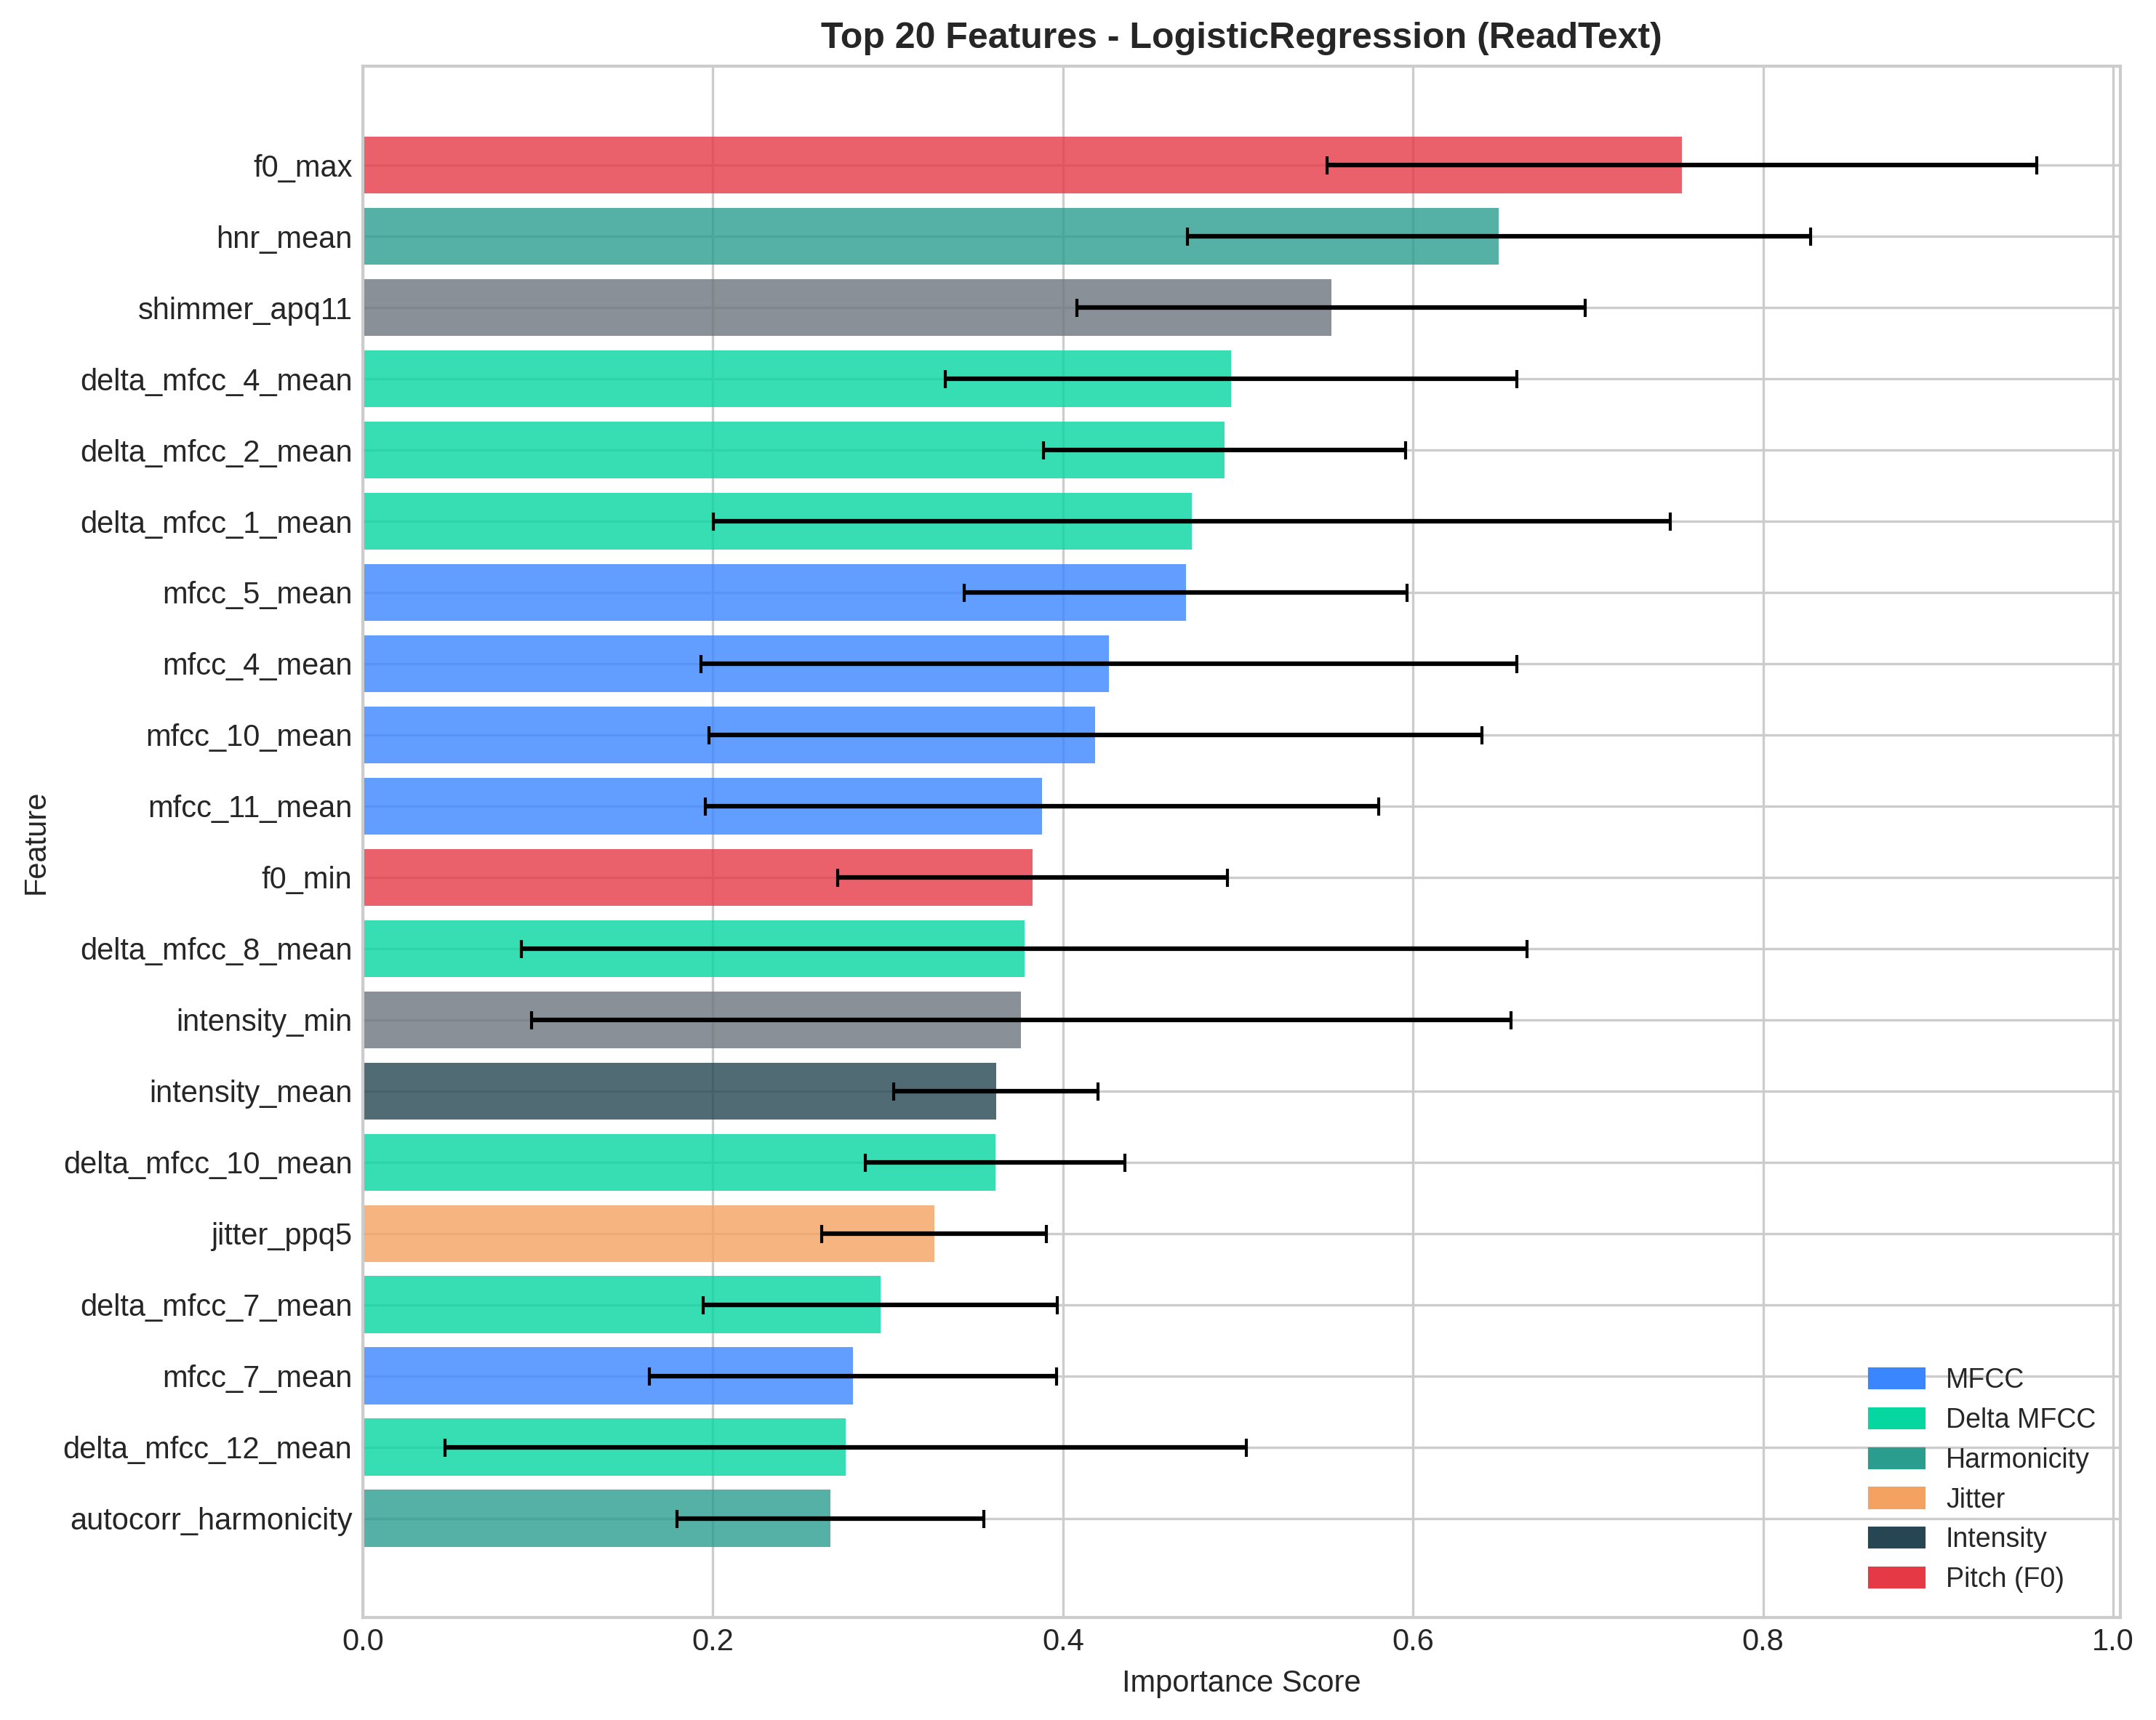
\includegraphics[width=0.8\textwidth]{figures/fig_imp_readtext_lr.png}
    \caption{Logistic Regression coefficient magnitudes (ReadText)}
    \label{fig:imp-readtext-lr}
\end{figure}

\subsection{Gradient Boosting --- Top 10 Features}

\begin{table}[H]
\centering
\begin{tabular}{@{}clcc@{}}
\toprule
\textbf{Rank} & \textbf{Feature} & \textbf{Importance} & \textbf{Std} \\
\midrule
1 & f0\_max & 0.229 & 0.179 \\
2 & mfcc\_4\_mean & 0.084 & 0.187 \\
3 & f1\_std & 0.080 & 0.178 \\
4 & mfcc\_6\_mean & 0.066 & 0.143 \\
5 & intensity\_min & 0.064 & 0.122 \\
6 & mfcc\_2\_mean & 0.060 & 0.133 \\
7 & f0\_std & 0.055 & 0.081 \\
8 & f3\_std & 0.054 & 0.070 \\
9 & delta\_mfcc\_10\_mean & 0.047 & 0.104 \\
10 & delta\_mfcc\_2\_mean & 0.041 & 0.083 \\
\bottomrule
\end{tabular}
\caption{Gradient Boosting feature importance --- ReadText (top 10)}
\label{tab:gb-readtext-importance}
\end{table}

\begin{figure}[H]
    \centering
    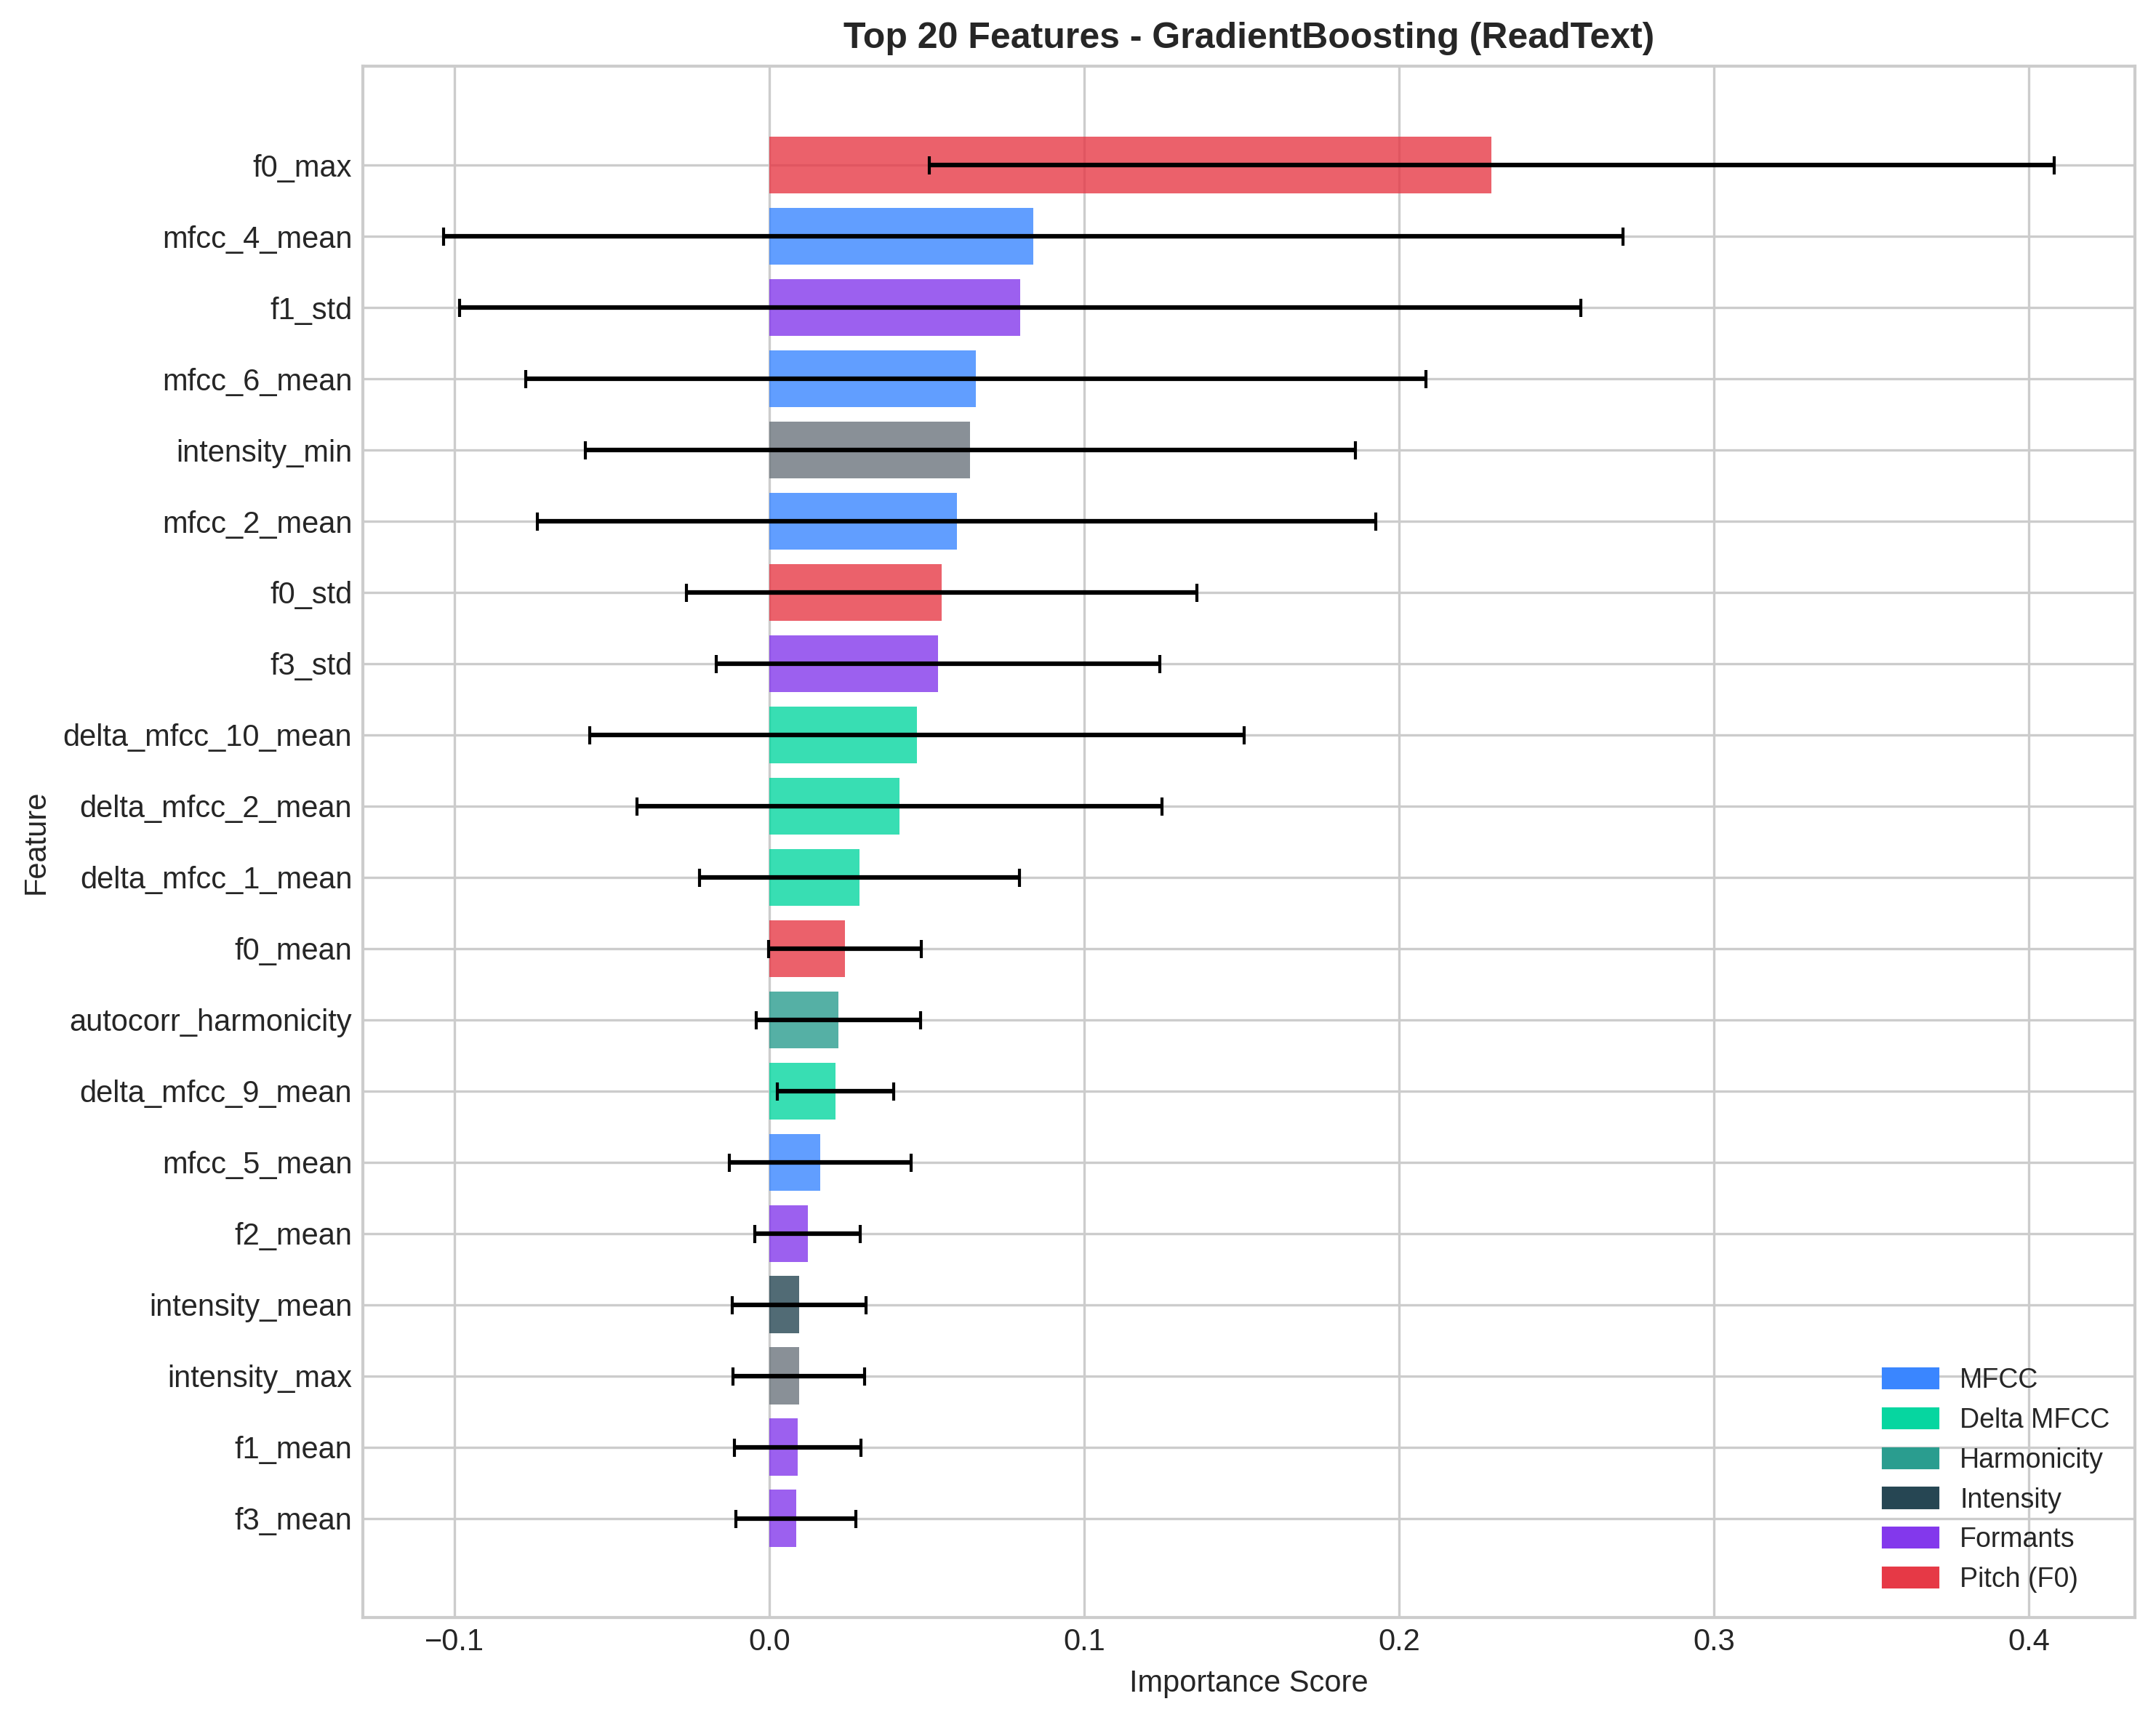
\includegraphics[width=0.8\textwidth]{fig_imp_readtext_gb.png}
    \caption{Gradient Boosting feature importances (ReadText). F0 max dominates strongly ($0.229 \pm 0.179$), consistent with pitch dysregulation in PD.}
    \label{fig:imp-readtext-gb}
\end{figure}

\subsection{XGBoost --- Top 10 Features}

\begin{table}[H]
\centering
\begin{tabular}{@{}clcc@{}}
\toprule
\textbf{Rank} & \textbf{Feature} & \textbf{Importance} & \textbf{Std} \\
\midrule
1 & f0\_max & 0.083 & 0.028 \\
2 & intensity\_min & 0.064 & 0.063 \\
3 & f0\_mean & 0.063 & 0.044 \\
4 & f3\_std & 0.061 & 0.044 \\
5 & intensity\_mean & 0.051 & 0.047 \\
6 & delta\_mfcc\_10\_mean & 0.041 & 0.037 \\
7 & f1\_std & 0.041 & 0.075 \\
8 & delta\_mfcc\_2\_mean & 0.038 & 0.028 \\
9 & mfcc\_3\_mean & 0.033 & 0.023 \\
10 & mfcc\_11\_mean & 0.031 & 0.040 \\
\bottomrule
\end{tabular}
\caption{XGBoost feature importance --- ReadText (top 10)}
\label{tab:xgb-readtext-importance}
\end{table}

\begin{figure}[H]
    \centering
    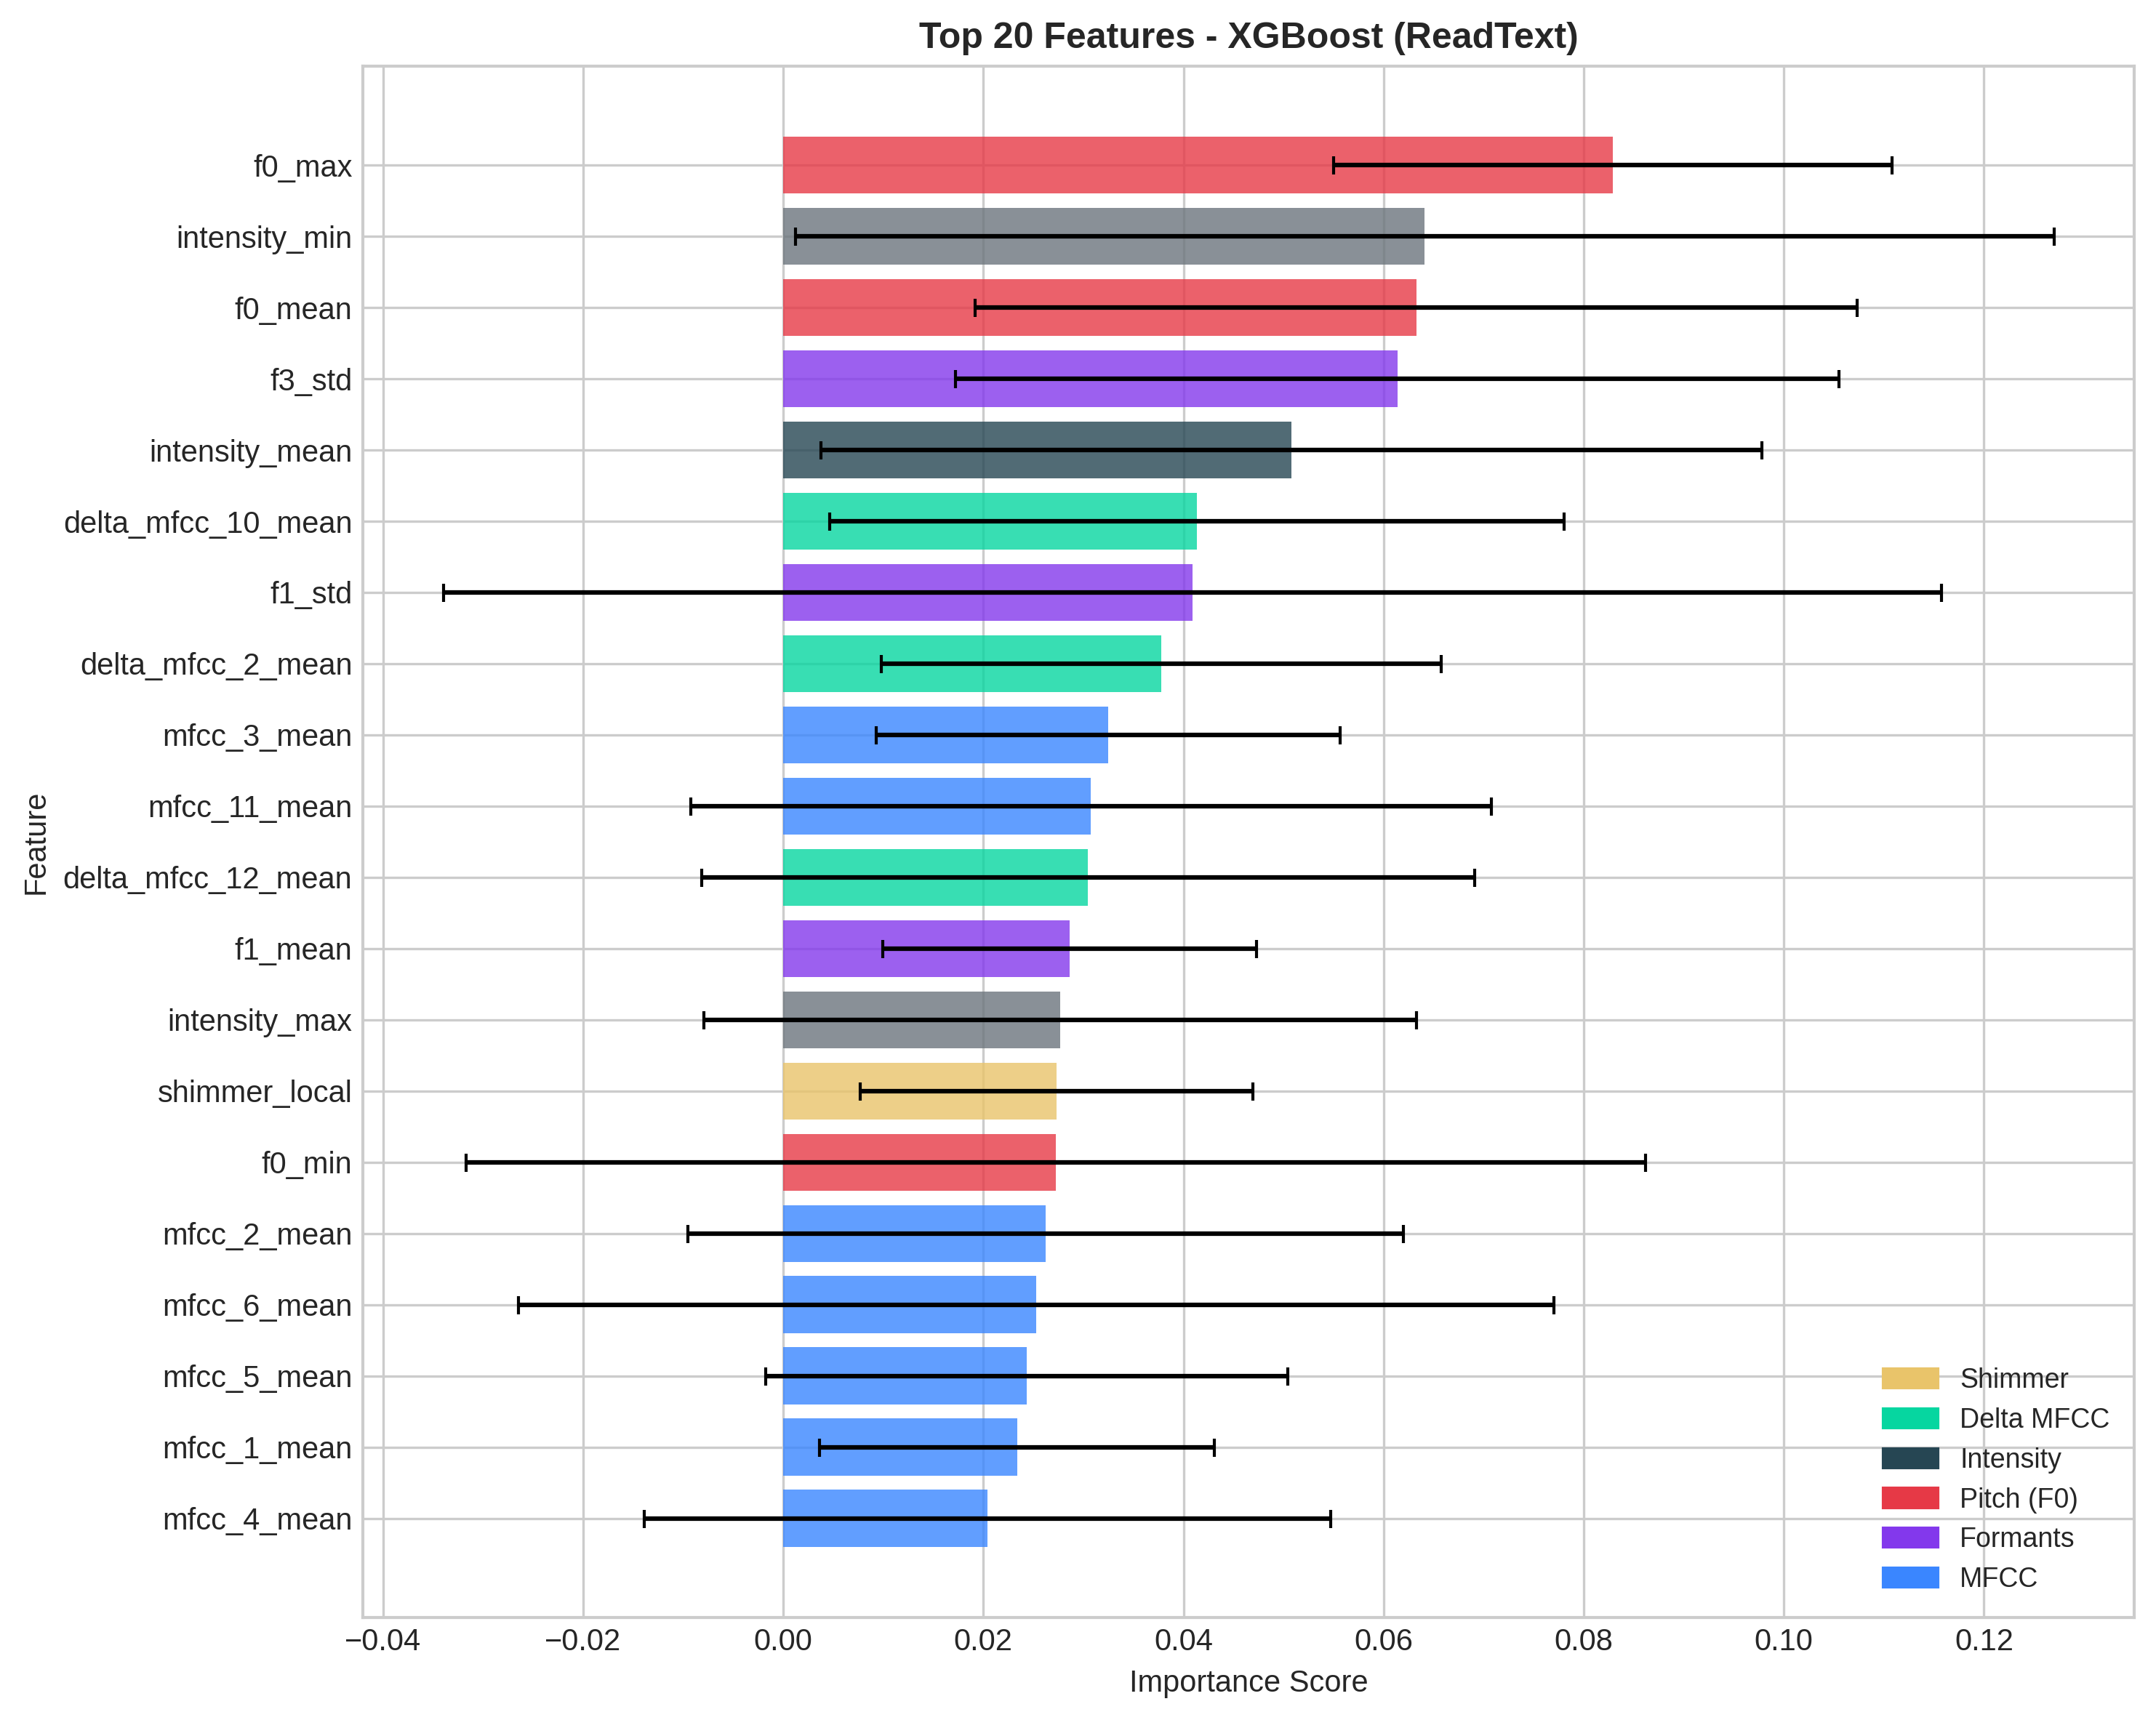
\includegraphics[width=0.8\textwidth]{fig_imp_readtext_xgb.png}
    \caption{XGBoost feature importances (ReadText). Importance is more distributed than Gradient Boosting, with F0 and intensity features sharing dominance.}
    \label{fig:imp-readtext-xgb}
\end{figure}

\section{Dataset A --- SpontaneousDialogue Task}

\subsection{Random Forest --- Top 20 Features}

\begin{table}[H]
\centering
\begin{tabular}{@{}clcc@{}}
\toprule
\textbf{Rank} & \textbf{Feature} & \textbf{Importance} & \textbf{Std} \\
\midrule
1 & mfcc\_5\_mean & 0.080 & 0.022 \\
2 & shimmer\_apq11 & 0.069 & 0.007 \\
3 & delta\_mfcc\_8\_mean & 0.051 & 0.015 \\
4 & jitter\_local & 0.041 & 0.012 \\
5 & delta\_mfcc\_2\_mean & 0.040 & 0.018 \\
6 & autocorr\_harmonicity & 0.037 & 0.011 \\
7 & shimmer\_local & 0.036 & 0.017 \\
8 & mfcc\_1\_mean & 0.034 & 0.010 \\
9 & f0\_std & 0.032 & 0.022 \\
10 & f0\_mean & 0.031 & 0.013 \\
\bottomrule
\end{tabular}
\caption{Random Forest feature importance --- SpontaneousDialogue (top 10)}
\label{tab:rf-spontaneous-importance}
\end{table}

\subsection{Logistic Regression --- Top 10 Features}

\begin{table}[H]
\centering
\begin{tabular}{@{}clcc@{}}
\toprule
\textbf{Rank} & \textbf{Feature} & \textbf{|Coefficient|} & \textbf{Std} \\
\midrule
1 & mfcc\_5\_mean & 0.722 & 0.039 \\
2 & delta\_mfcc\_8\_mean & 0.615 & 0.121 \\
3 & shimmer\_apq11 & 0.559 & 0.136 \\
4 & delta\_mfcc\_2\_mean & 0.493 & 0.196 \\
5 & intensity\_min & 0.459 & 0.170 \\
6 & mfcc\_3\_mean & 0.388 & 0.271 \\
7 & delta\_mfcc\_11\_mean & 0.381 & 0.102 \\
8 & delta\_mfcc\_7\_mean & 0.380 & 0.150 \\
9 & hnr\_mean & 0.379 & 0.175 \\
10 & delta\_mfcc\_1\_mean & 0.352 & 0.123 \\
\bottomrule
\end{tabular}
\caption{Logistic Regression feature importance --- SpontaneousDialogue (top 10)}
\label{tab:lr-spontaneous-importance}
\end{table}

\begin{figure}[H]
    \centering
    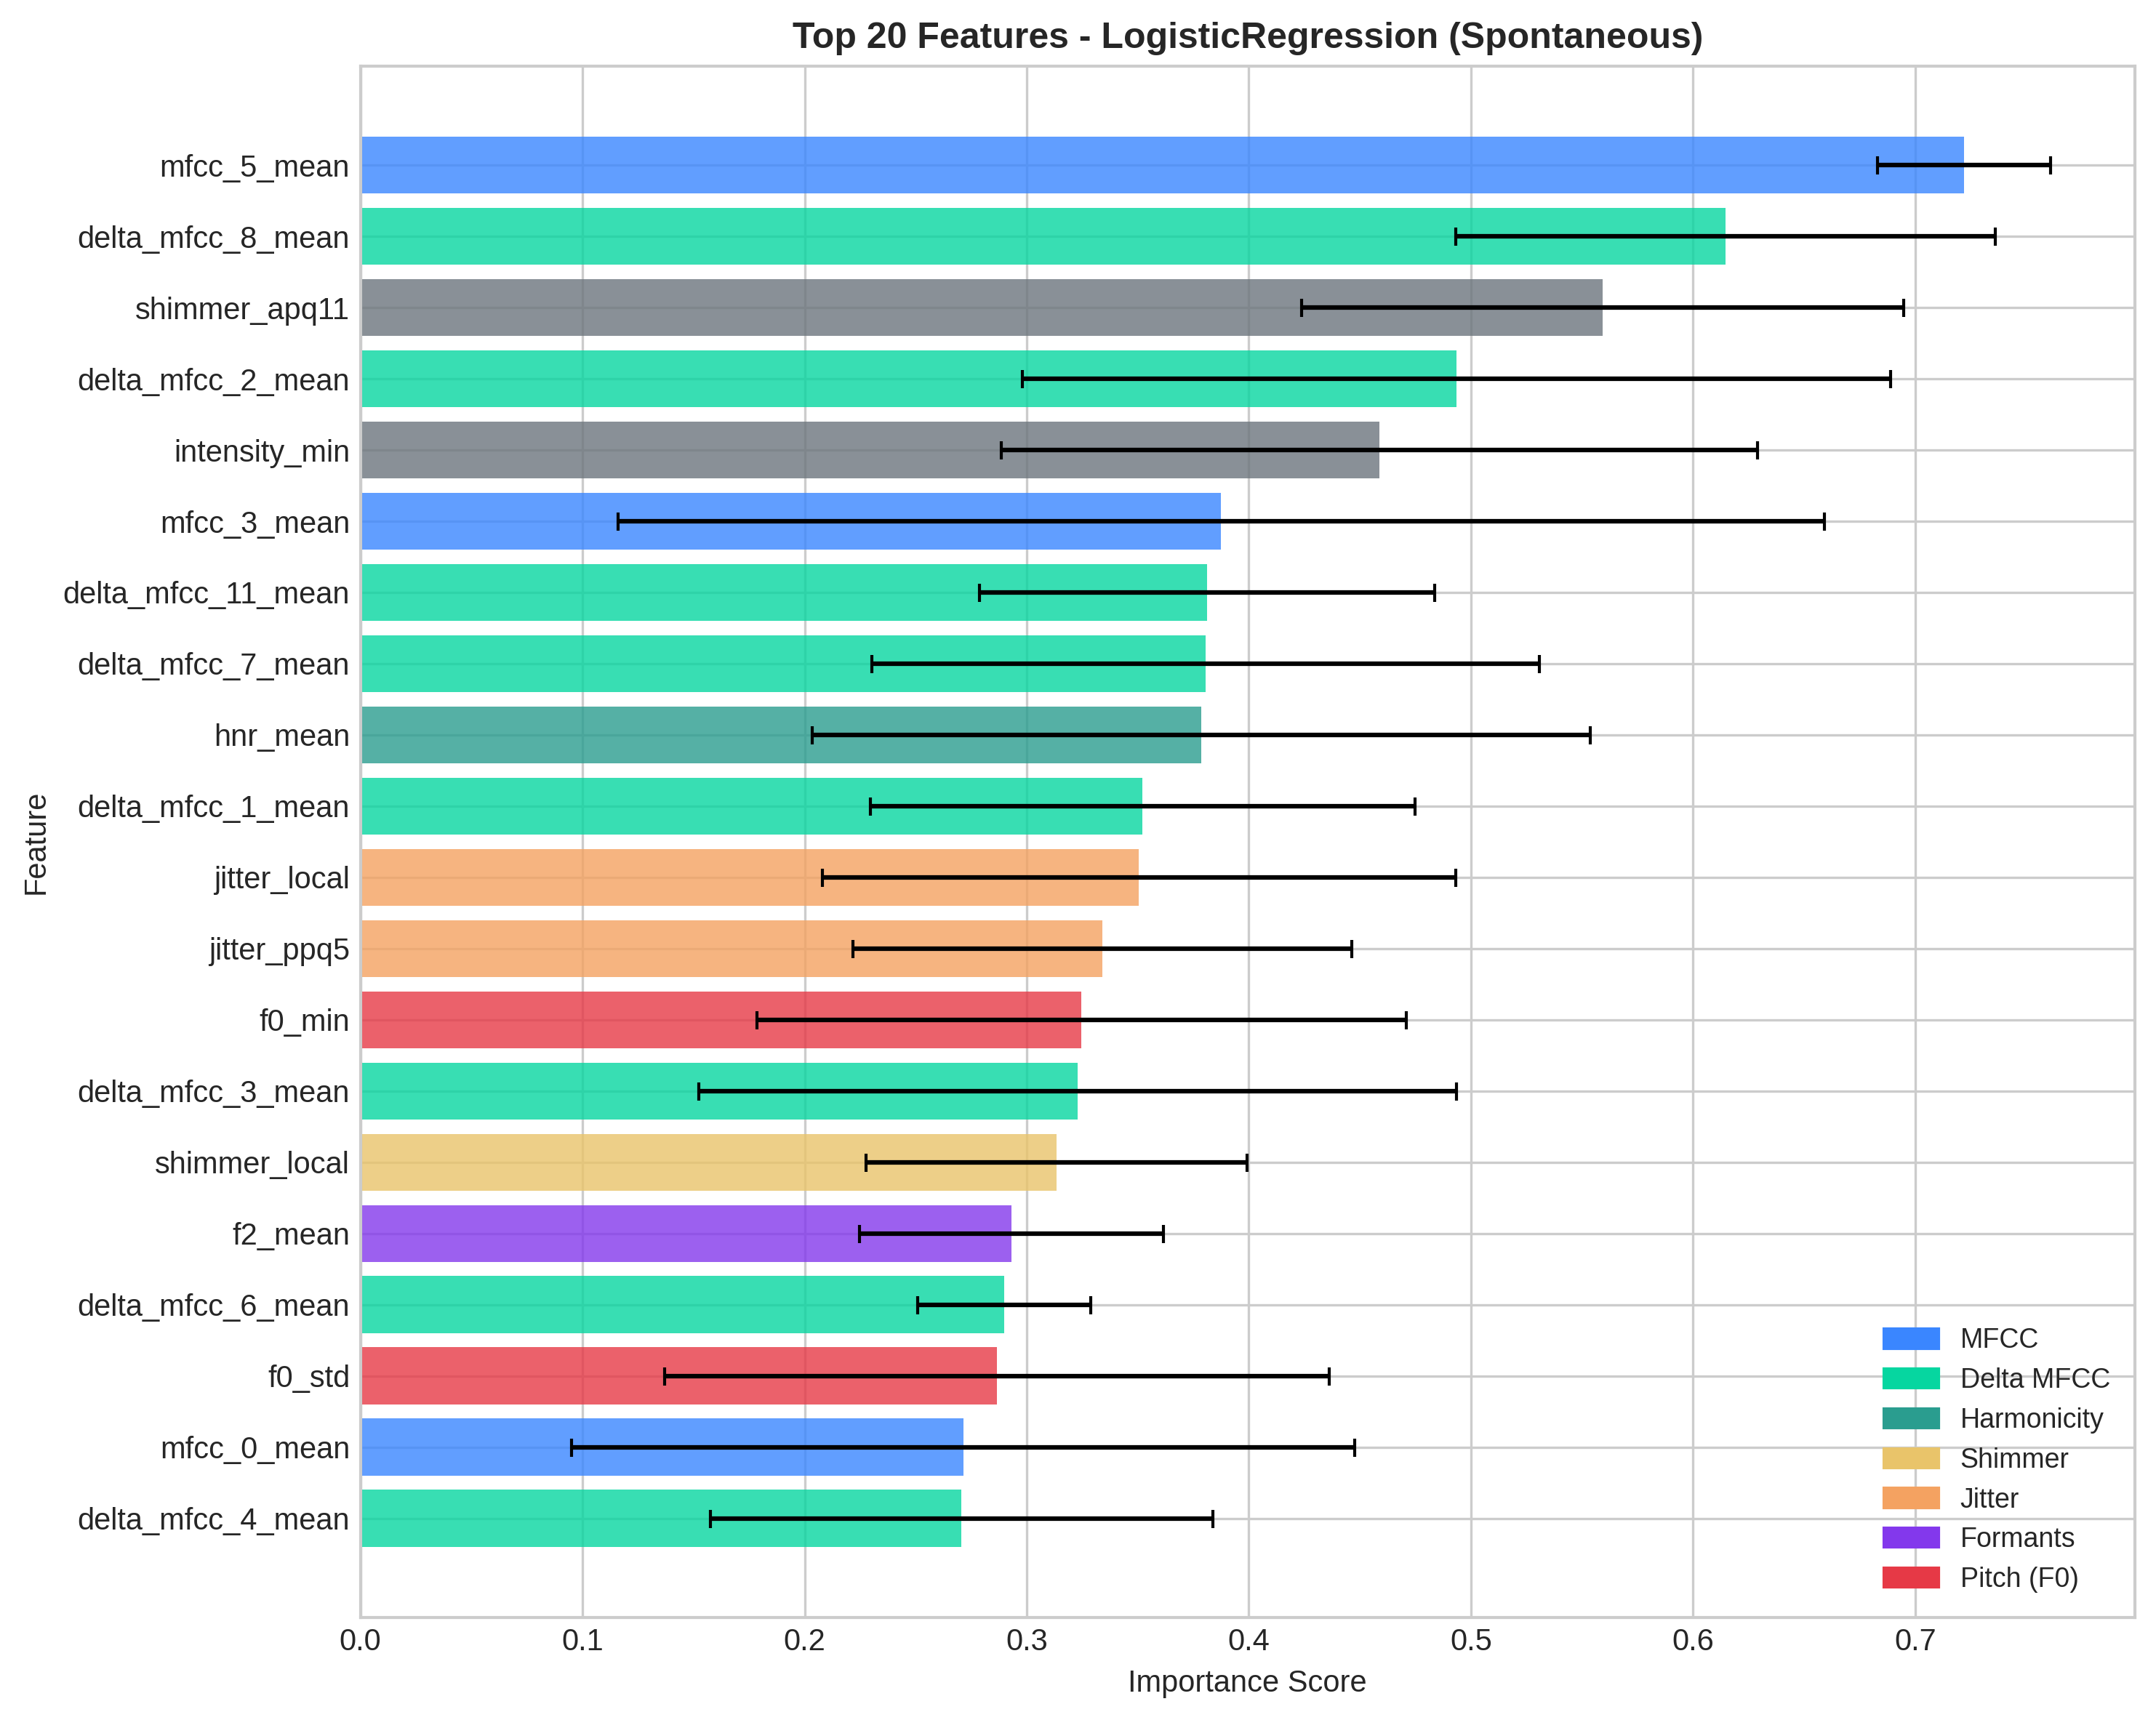
\includegraphics[width=0.8\textwidth]{figures/fig_imp_spontaneous_lr.png}
    \caption{Logistic Regression coefficient magnitudes (Spontaneous Dialogue)}
    \label{fig:imp-spontaneous-lr}
\end{figure}

\subsection{Gradient Boosting --- Top 10 Features}

\begin{table}[H]
\centering
\begin{tabular}{@{}clcc@{}}
\toprule
\textbf{Rank} & \textbf{Feature} & \textbf{Importance} & \textbf{Std} \\
\midrule
1 & mfcc\_5\_mean & 0.342 & 0.204 \\
2 & shimmer\_apq11 & 0.134 & 0.132 \\
3 & delta\_mfcc\_8\_mean & 0.086 & 0.192 \\
4 & intensity\_min & 0.050 & 0.093 \\
5 & shimmer\_local & 0.050 & 0.089 \\
6 & f1\_std & 0.040 & 0.033 \\
7 & mfcc\_11\_mean & 0.040 & 0.089 \\
8 & mfcc\_10\_mean & 0.027 & 0.020 \\
9 & mfcc\_1\_mean & 0.024 & 0.026 \\
10 & intensity\_max & 0.024 & 0.037 \\
\bottomrule
\end{tabular}
\caption{Gradient Boosting feature importance --- SpontaneousDialogue (top 10)}
\label{tab:gb-spontaneous-importance}
\end{table}

\begin{figure}[H]
    \centering
    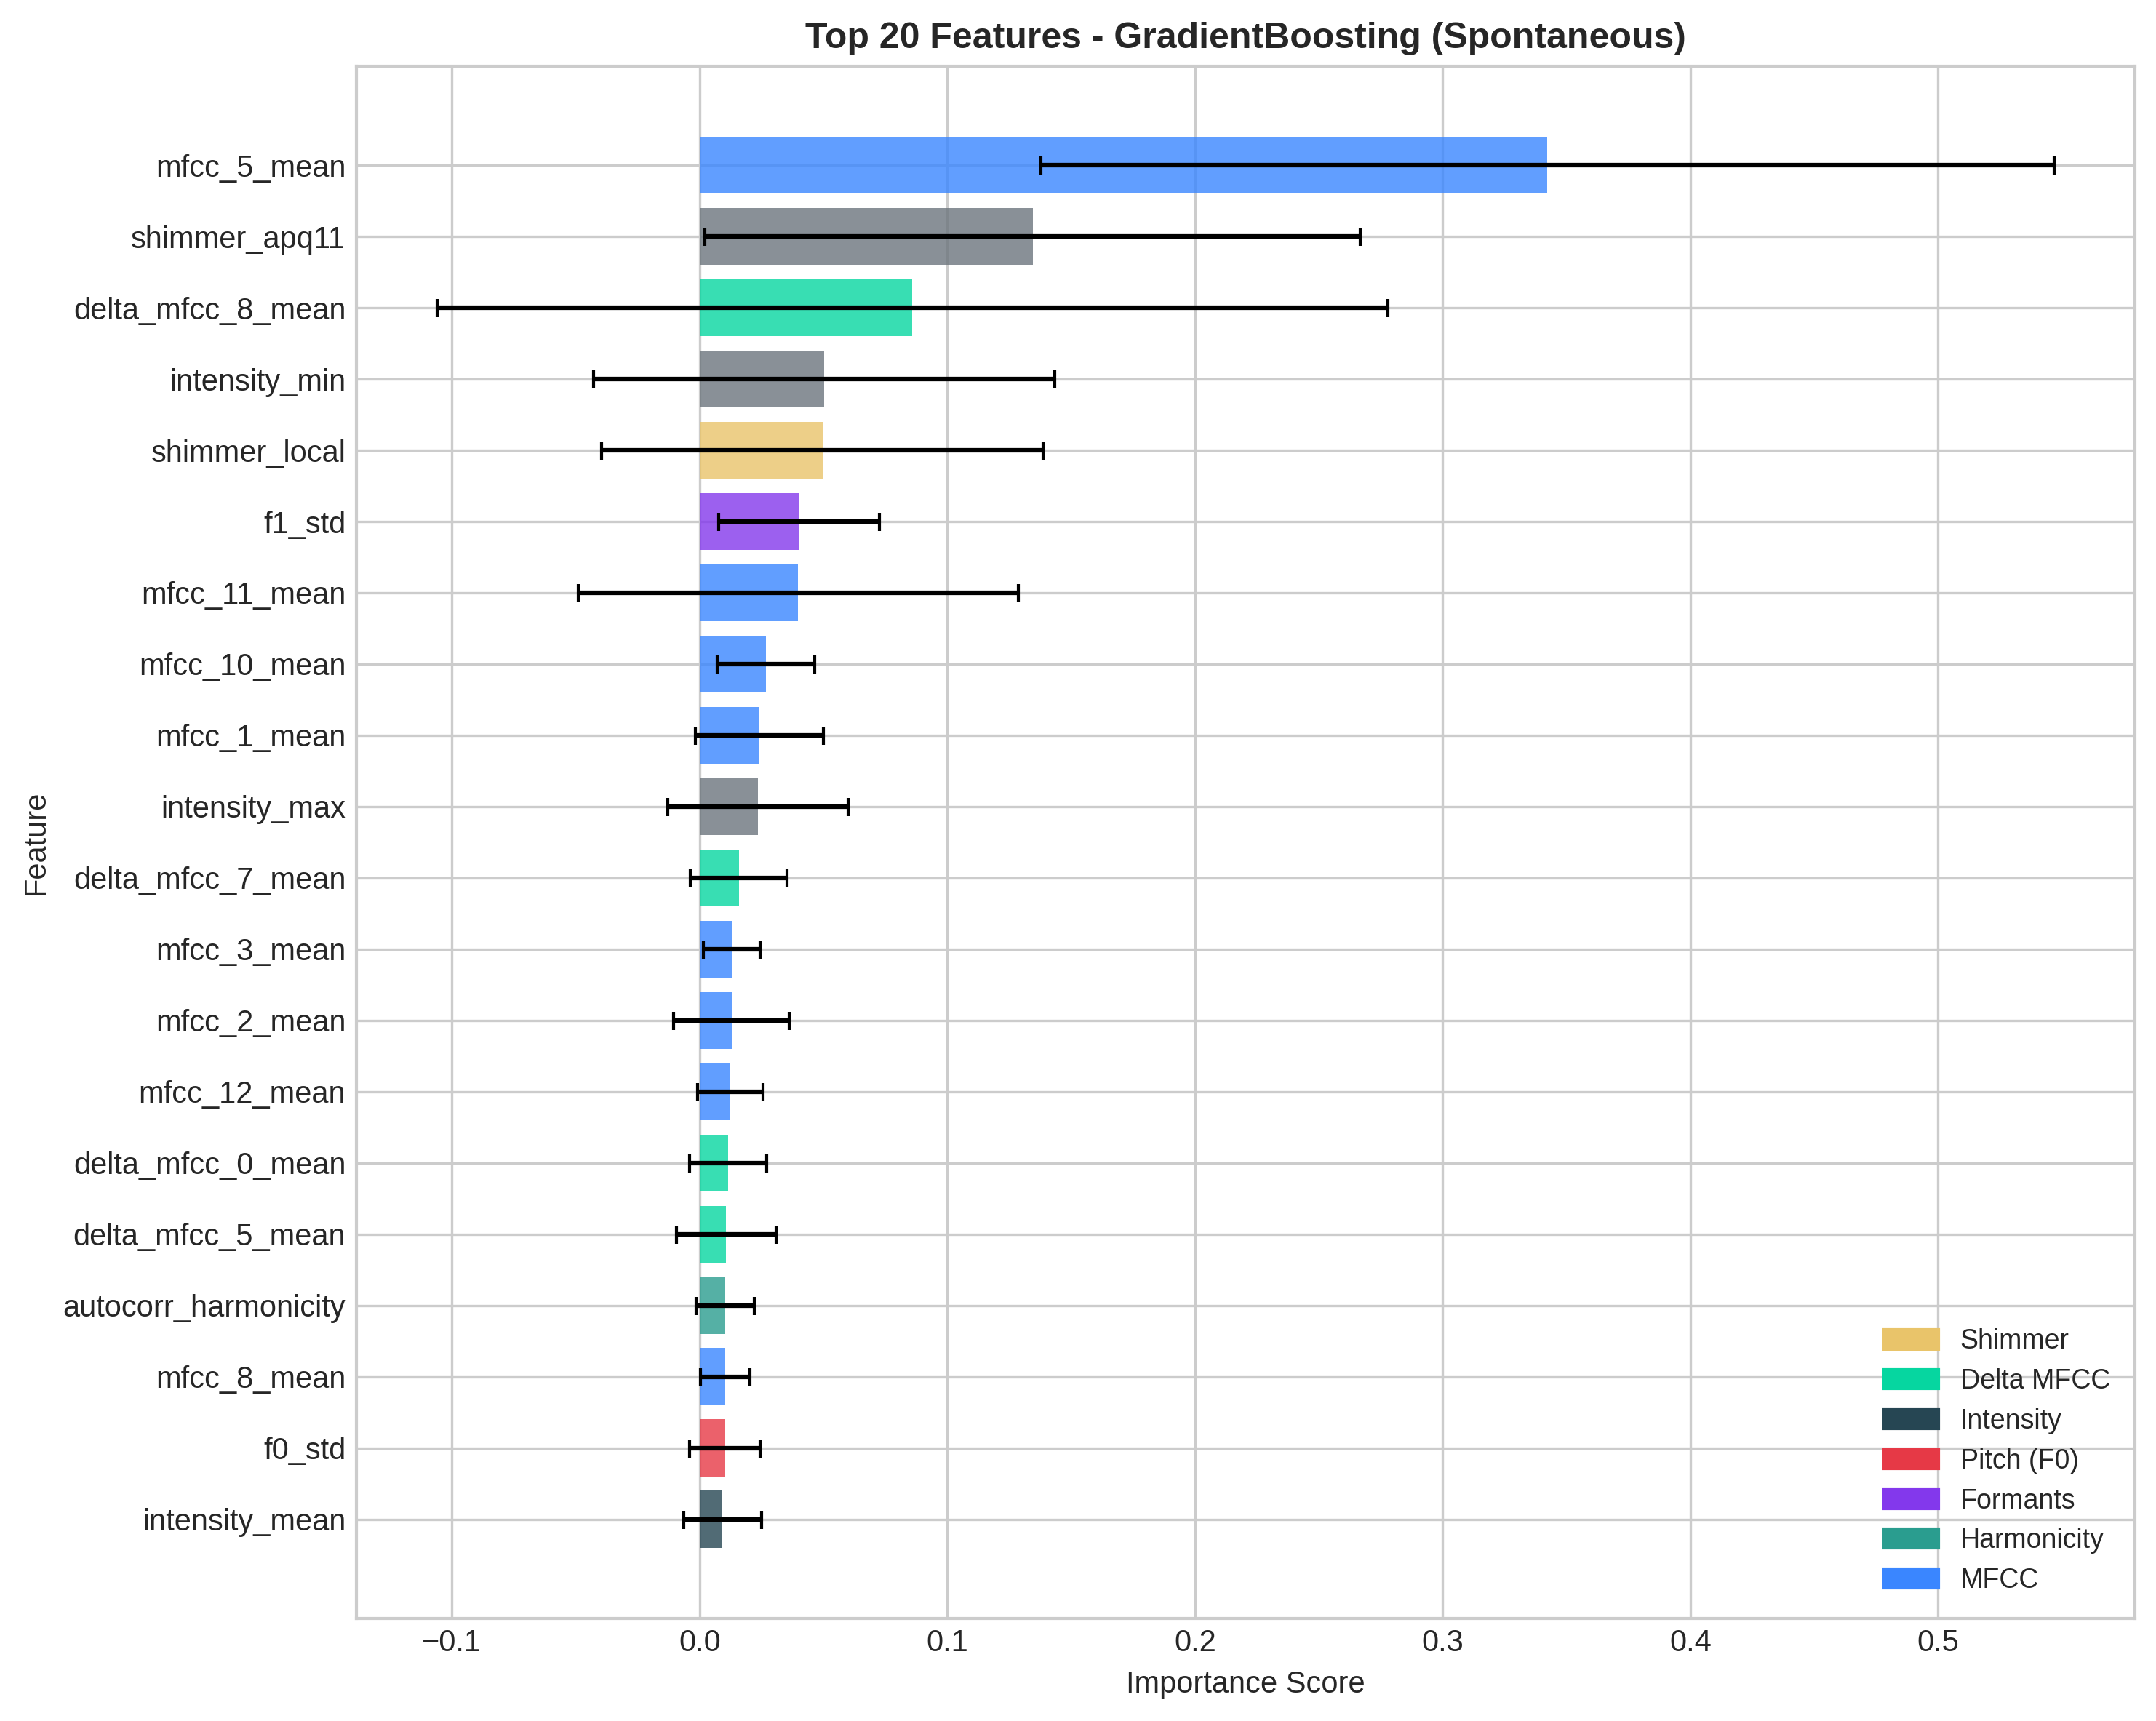
\includegraphics[width=0.8\textwidth]{fig_imp_spontaneous_gb.png}
    \caption{Gradient Boosting feature importances (Spontaneous Dialogue). MFCC-5 ($0.342 \pm 0.204$) strongly dominates, reflecting spectral tilt changes in spontaneous PD speech.}
    \label{fig:imp-spontaneous-gb}
\end{figure}

\subsection{XGBoost --- Top 10 Features}

\begin{table}[H]
\centering
\begin{tabular}{@{}clcc@{}}
\toprule
\textbf{Rank} & \textbf{Feature} & \textbf{Importance} & \textbf{Std} \\
\midrule
1 & mfcc\_5\_mean & 0.134 & 0.059 \\
2 & shimmer\_apq11 & 0.104 & 0.071 \\
3 & delta\_mfcc\_8\_mean & 0.079 & 0.052 \\
4 & delta\_mfcc\_2\_mean & 0.053 & 0.009 \\
5 & mfcc\_4\_mean & 0.035 & 0.022 \\
6 & mfcc\_2\_mean & 0.033 & 0.022 \\
7 & jitter\_local & 0.032 & 0.012 \\
8 & f0\_mean & 0.031 & 0.035 \\
9 & shimmer\_local & 0.031 & 0.054 \\
10 & intensity\_max & 0.030 & 0.030 \\
\bottomrule
\end{tabular}
\caption{XGBoost feature importance --- SpontaneousDialogue (top 10)}
\label{tab:xgb-spontaneous-importance}
\end{table}

\begin{figure}[H]
    \centering
    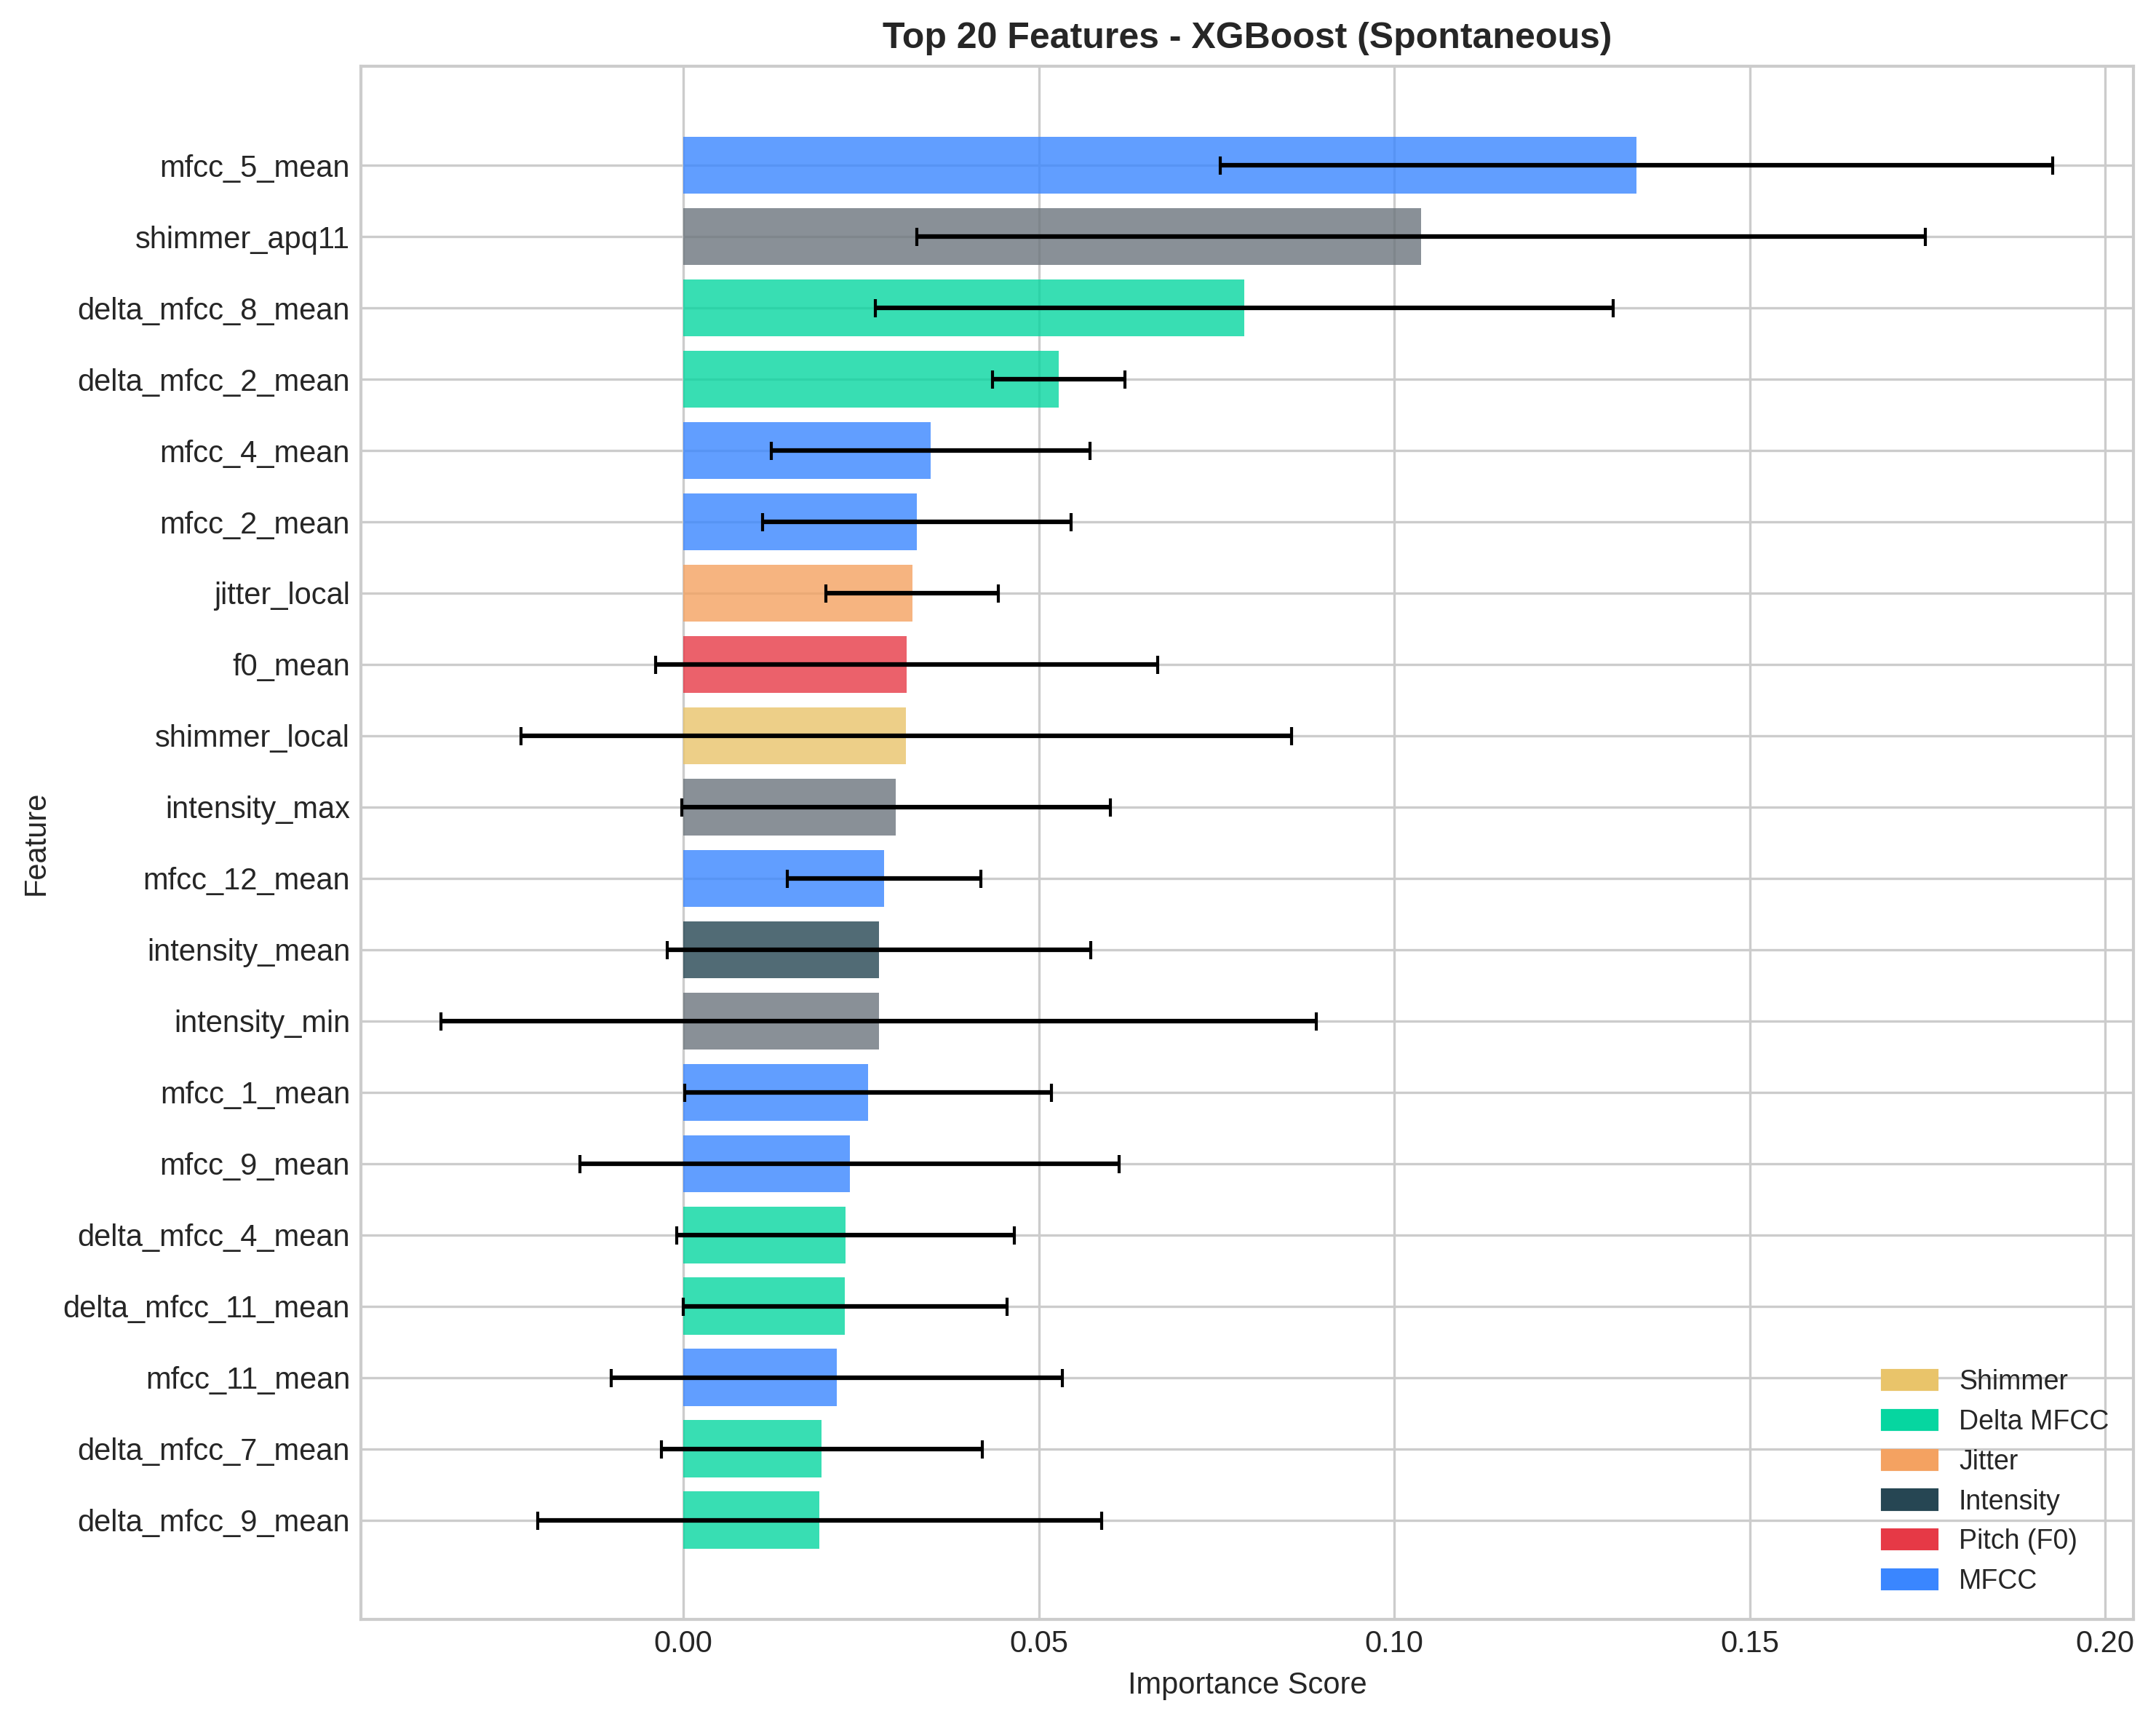
\includegraphics[width=0.8\textwidth]{fig_imp_spontaneous_xgb.png}
    \caption{XGBoost feature importances (Spontaneous Dialogue). MFCC-5 and shimmer features dominate, consistent with RF and GB findings for this task.}
    \label{fig:imp-spontaneous-xgb}
\end{figure}

\section{Dataset B --- PD Speech Features}

Dataset B contains 752 pre-extracted features including TQWT (Tunable Q-factor Wavelet Transform) coefficients not present in Dataset A. Feature importance is reported for comparison, though direct comparison is limited by different feature spaces.

\subsection{Random Forest --- Top 10 Features}

\begin{table}[H]
\centering
\begin{tabular}{@{}clcc@{}}
\toprule
\textbf{Rank} & \textbf{Feature} & \textbf{Importance} & \textbf{Std} \\
\midrule
1 & std\_delta\_log\_energy & 0.013 & 0.004 \\
2 & std\_delta\_delta\_log\_energy & 0.013 & 0.003 \\
3 & tqwt\_entropy\_shannon\_dec\_12 & 0.012 & 0.001 \\
4 & tqwt\_TKEO\_std\_dec\_11 & 0.010 & 0.004 \\
5 & tqwt\_TKEO\_mean\_dec\_12 & 0.010 & 0.001 \\
6 & mean\_MFCC\_2nd\_coef & 0.008 & 0.003 \\
7 & tqwt\_entropy\_log\_dec\_11 & 0.008 & 0.003 \\
8 & tqwt\_stdValue\_dec\_12 & 0.008 & 0.003 \\
9 & tqwt\_stdValue\_dec\_13 & 0.008 & 0.003 \\
10 & tqwt\_energy\_dec\_12 & 0.007 & 0.003 \\
\bottomrule
\end{tabular}
\caption{Random Forest feature importance --- Dataset B (top 10)}
\label{tab:rf-datasetb-importance}
\end{table}

\textbf{Note:} Importance values are lower than Dataset A due to the larger feature space (752 vs 47 features), distributing importance more broadly.

\subsection{Logistic Regression --- Top 10 Features}

\begin{table}[H]
\centering
\begin{tabular}{@{}clcc@{}}
\toprule
\textbf{Rank} & \textbf{Feature} & \textbf{|Coefficient|} & \textbf{Std} \\
\midrule
1 & tqwt\_kurtosisValue\_dec\_33 & 0.733 & 0.161 \\
2 & tqwt\_entropy\_log\_dec\_33 & 0.694 & 0.084 \\
3 & mean\_MFCC\_7th\_coef & 0.614 & 0.148 \\
4 & std\_delta\_delta\_log\_energy & 0.588 & 0.133 \\
5 & std\_MFCC\_2nd\_coef & 0.567 & 0.202 \\
6 & tqwt\_meanValue\_dec\_16 & 0.551 & 0.114 \\
7 & tqwt\_medianValue\_dec\_25 & 0.540 & 0.209 \\
8 & mean\_MFCC\_3rd\_coef & 0.538 & 0.155 \\
9 & tqwt\_meanValue\_dec\_22 & 0.528 & 0.172 \\
10 & std\_9th\_delta & 0.526 & 0.103 \\
\bottomrule
\end{tabular}
\caption{Logistic Regression feature importance --- Dataset B (top 10)}
\label{tab:lr-datasetb-importance}
\end{table}

\textbf{Observation:} TQWT features dominate Dataset B importance, reflecting the sustained vowel /a/ phonation task where time-frequency decomposition captures subtle vocal tremor patterns.

\begin{figure}[H]
    \centering
    \begin{subfigure}[b]{0.48\textwidth}
        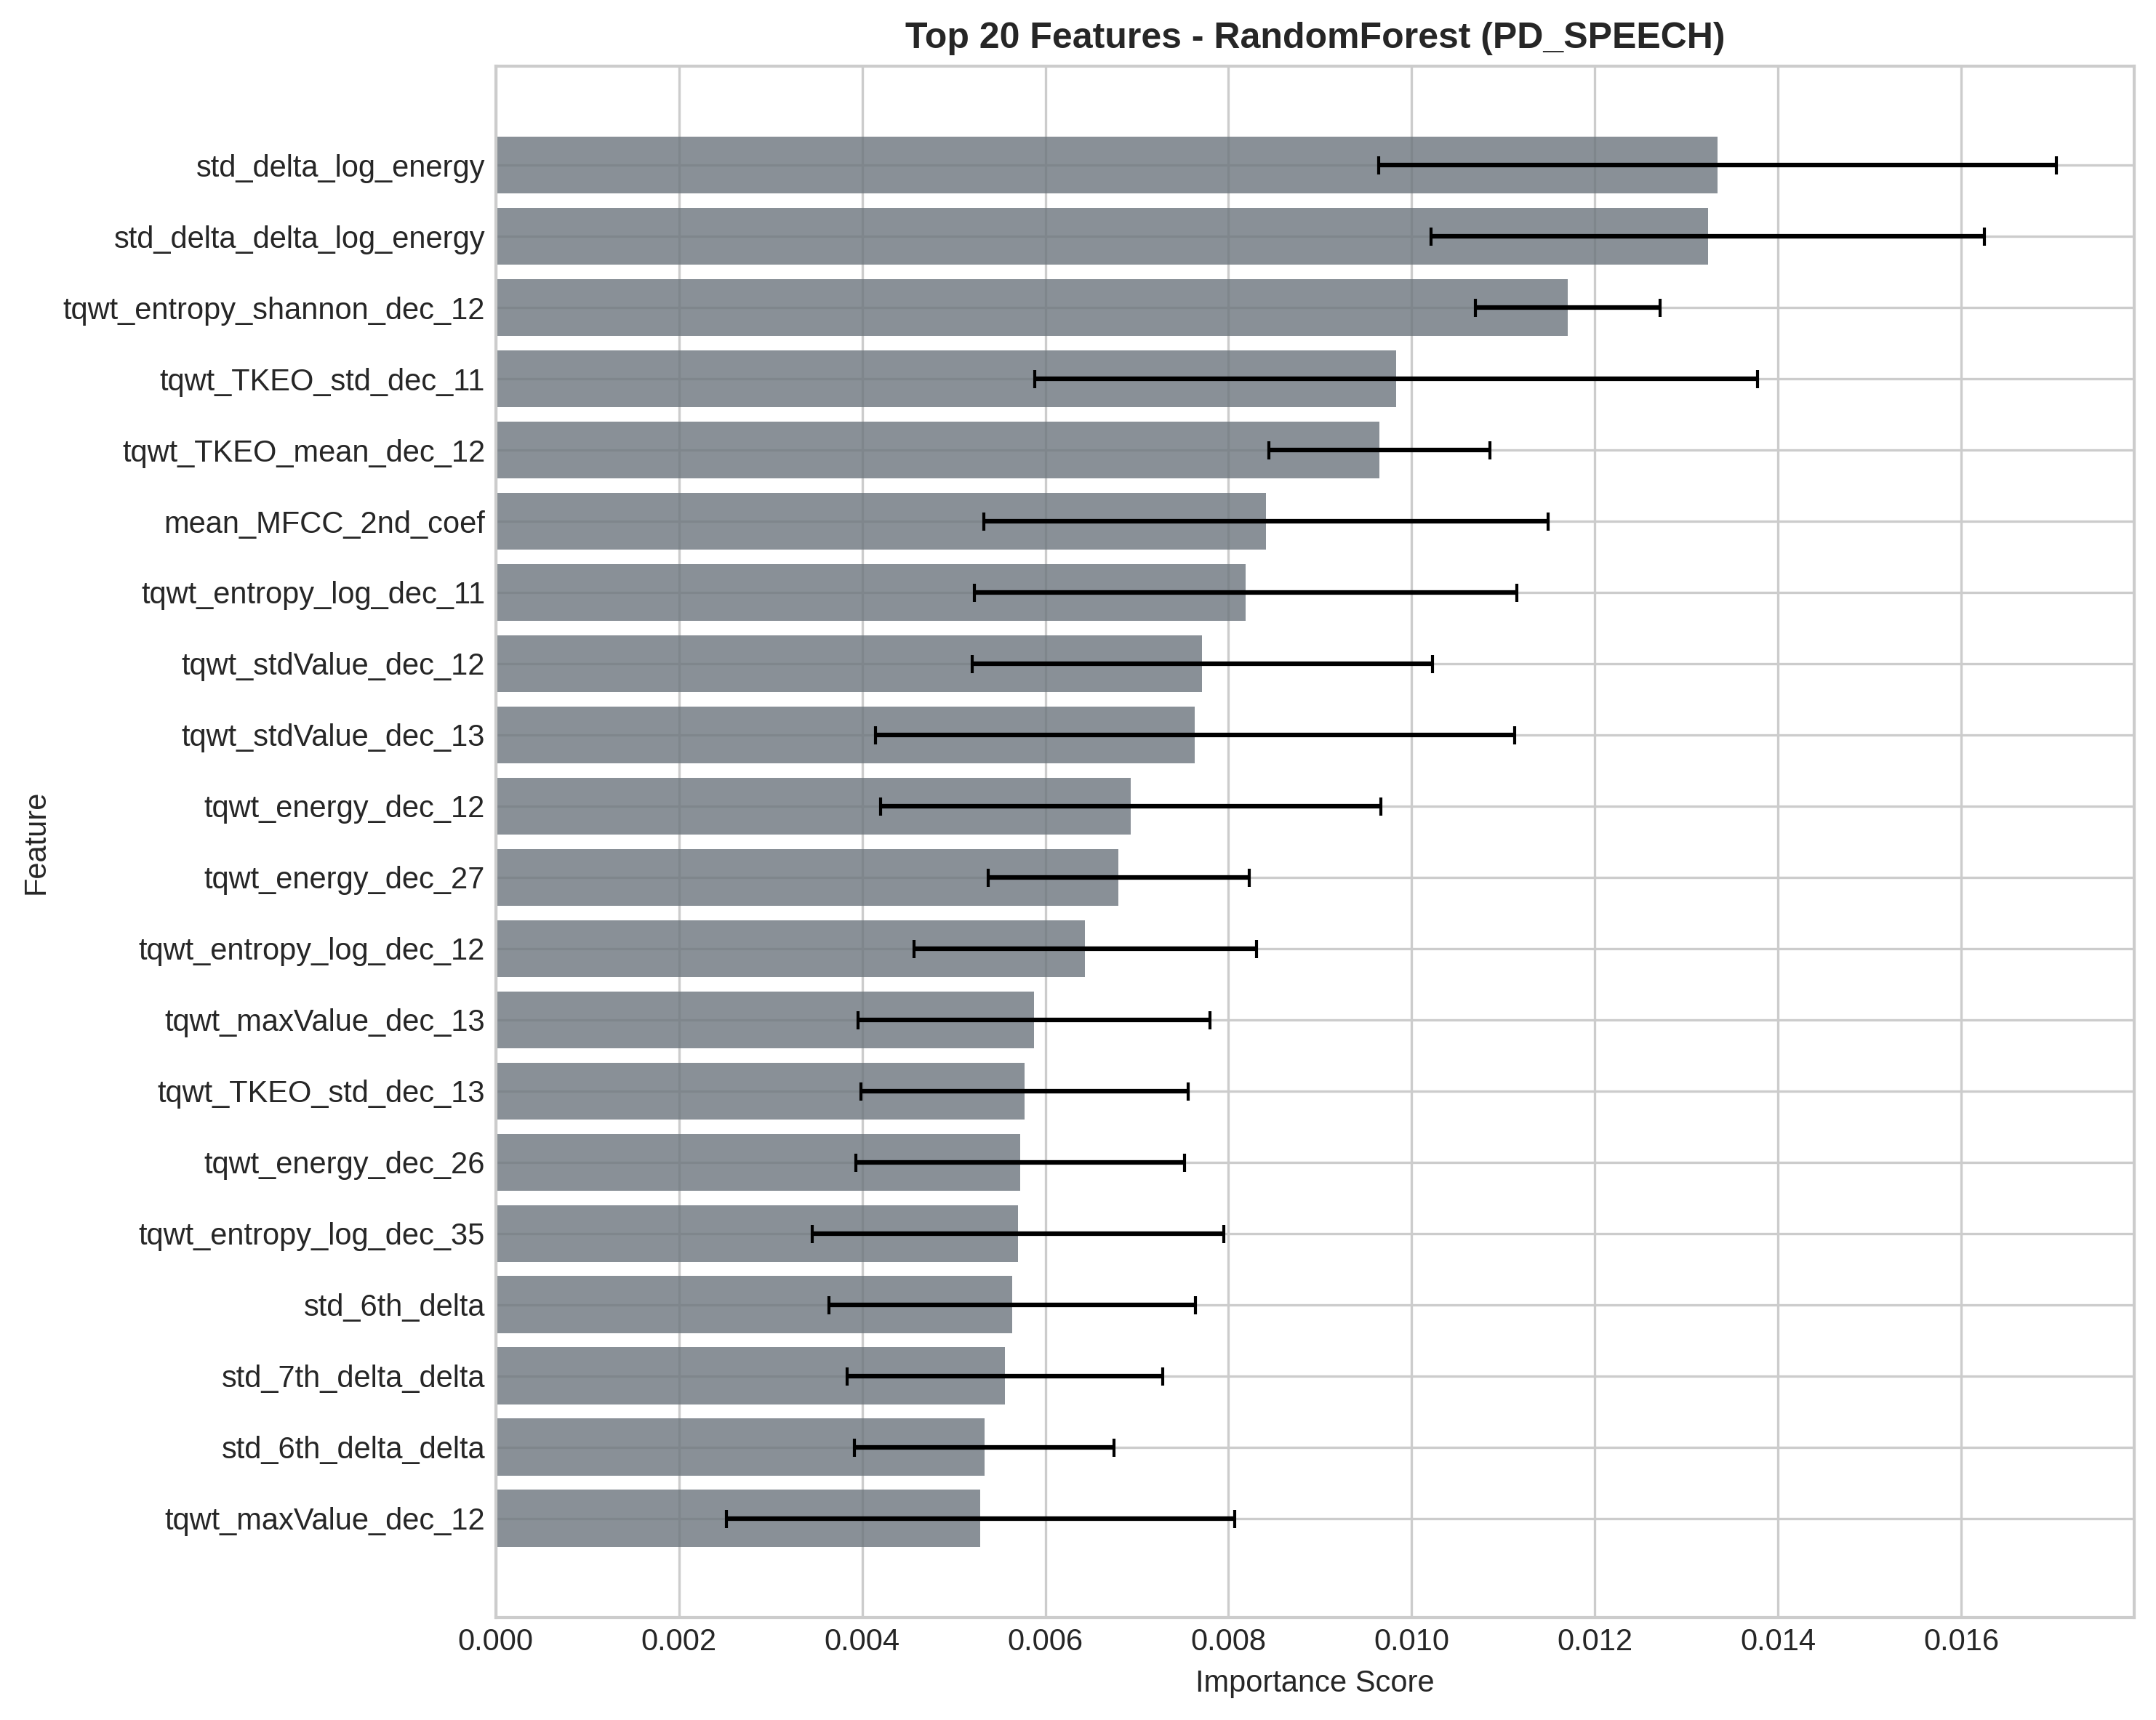
\includegraphics[width=\textwidth]{fig_imp_datasetb_rf.png}
        \caption{Random Forest}
        \label{fig:imp-datasetb-rf}
    \end{subfigure}
    \hfill
    \begin{subfigure}[b]{0.48\textwidth}
        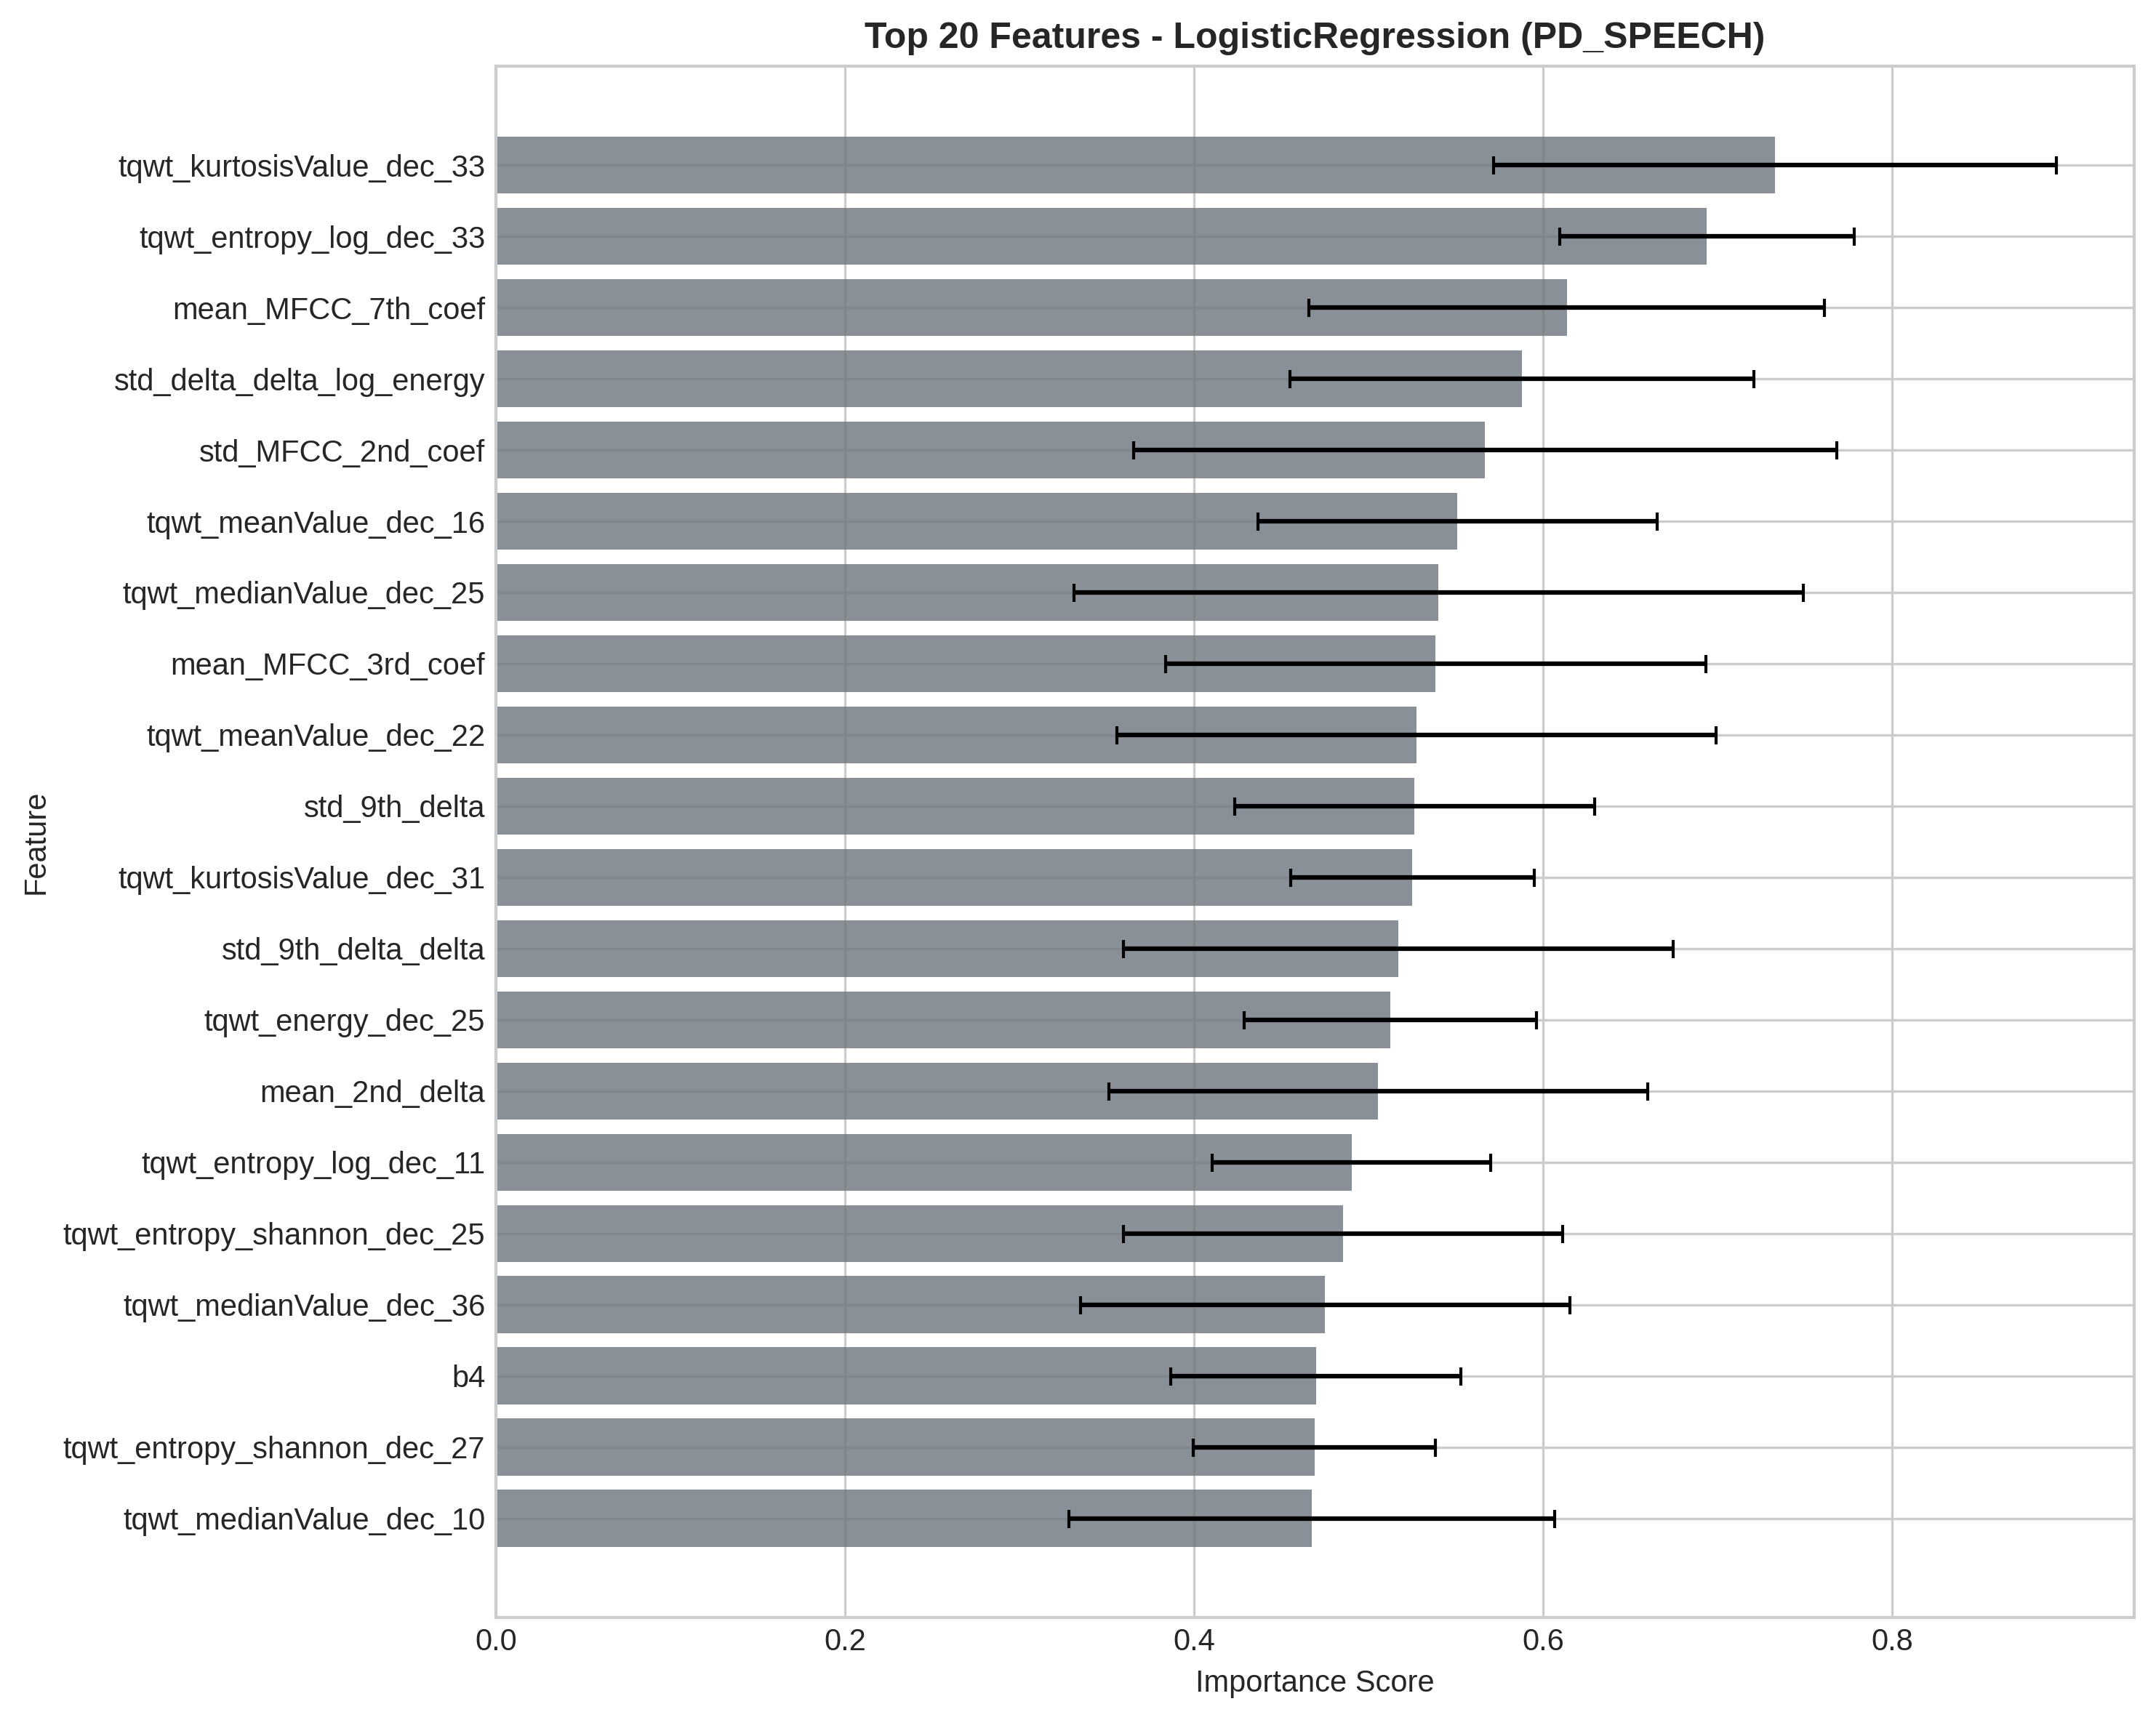
\includegraphics[width=\textwidth]{fig_imp_datasetb_lr.png}
        \caption{Logistic Regression}
        \label{fig:imp-datasetb-lr}
    \end{subfigure}
    \caption{Feature importance for Dataset B (PD Speech Features) --- Random Forest and Logistic Regression.}
    \label{fig:imp-datasetb}
\end{figure}

\subsection{Gradient Boosting --- Top 10 Features}

\begin{table}[H]
\centering
\begin{tabular}{@{}clcc@{}}
\toprule
\textbf{Rank} & \textbf{Feature} & \textbf{Importance} & \textbf{Std} \\
\midrule
1 & std\_delta\_delta\_log\_energy & 0.133 & 0.035 \\
2 & tqwt\_TKEO\_mean\_dec\_12 & 0.030 & 0.036 \\
3 & tqwt\_entropy\_log\_dec\_27 & 0.029 & 0.008 \\
4 & std\_7th\_delta\_delta & 0.028 & 0.005 \\
5 & tqwt\_energy\_dec\_27 & 0.024 & 0.028 \\
6 & tqwt\_entropy\_log\_dec\_35 & 0.023 & 0.019 \\
7 & tqwt\_TKEO\_std\_dec\_12 & 0.023 & 0.026 \\
8 & mean\_MFCC\_2nd\_coef & 0.021 & 0.024 \\
9 & tqwt\_entropy\_log\_dec\_33 & 0.021 & 0.006 \\
10 & tqwt\_TKEO\_std\_dec\_11 & 0.020 & 0.021 \\
\bottomrule
\end{tabular}
\caption{Gradient Boosting feature importance --- Dataset B (top 10)}
\label{tab:gb-datasetb-importance}
\end{table}

\subsection{XGBoost --- Top 10 Features}

\begin{table}[H]
\centering
\begin{tabular}{@{}clcc@{}}
\toprule
\textbf{Rank} & \textbf{Feature} & \textbf{Importance} & \textbf{Std} \\
\midrule
1 & tqwt\_entropy\_log\_dec\_12 & 0.024 & 0.020 \\
2 & std\_delta\_delta\_log\_energy & 0.017 & 0.006 \\
3 & tqwt\_TKEO\_mean\_dec\_12 & 0.016 & 0.017 \\
4 & tqwt\_TKEO\_std\_dec\_12 & 0.013 & 0.014 \\
5 & tqwt\_energy\_dec\_27 & 0.012 & 0.024 \\
6 & tqwt\_TKEO\_std\_dec\_11 & 0.012 & 0.010 \\
7 & tqwt\_entropy\_log\_dec\_16 & 0.010 & 0.009 \\
8 & tqwt\_entropy\_log\_dec\_13 & 0.009 & 0.012 \\
9 & mean\_MFCC\_2nd\_coef & 0.008 & 0.004 \\
10 & tqwt\_entropy\_shannon\_dec\_16 & 0.008 & 0.011 \\
\bottomrule
\end{tabular}
\caption{XGBoost feature importance --- Dataset B (top 10)}
\label{tab:xgb-datasetb-importance}
\end{table}

\begin{figure}[H]
    \centering
    \begin{subfigure}[b]{0.48\textwidth}
        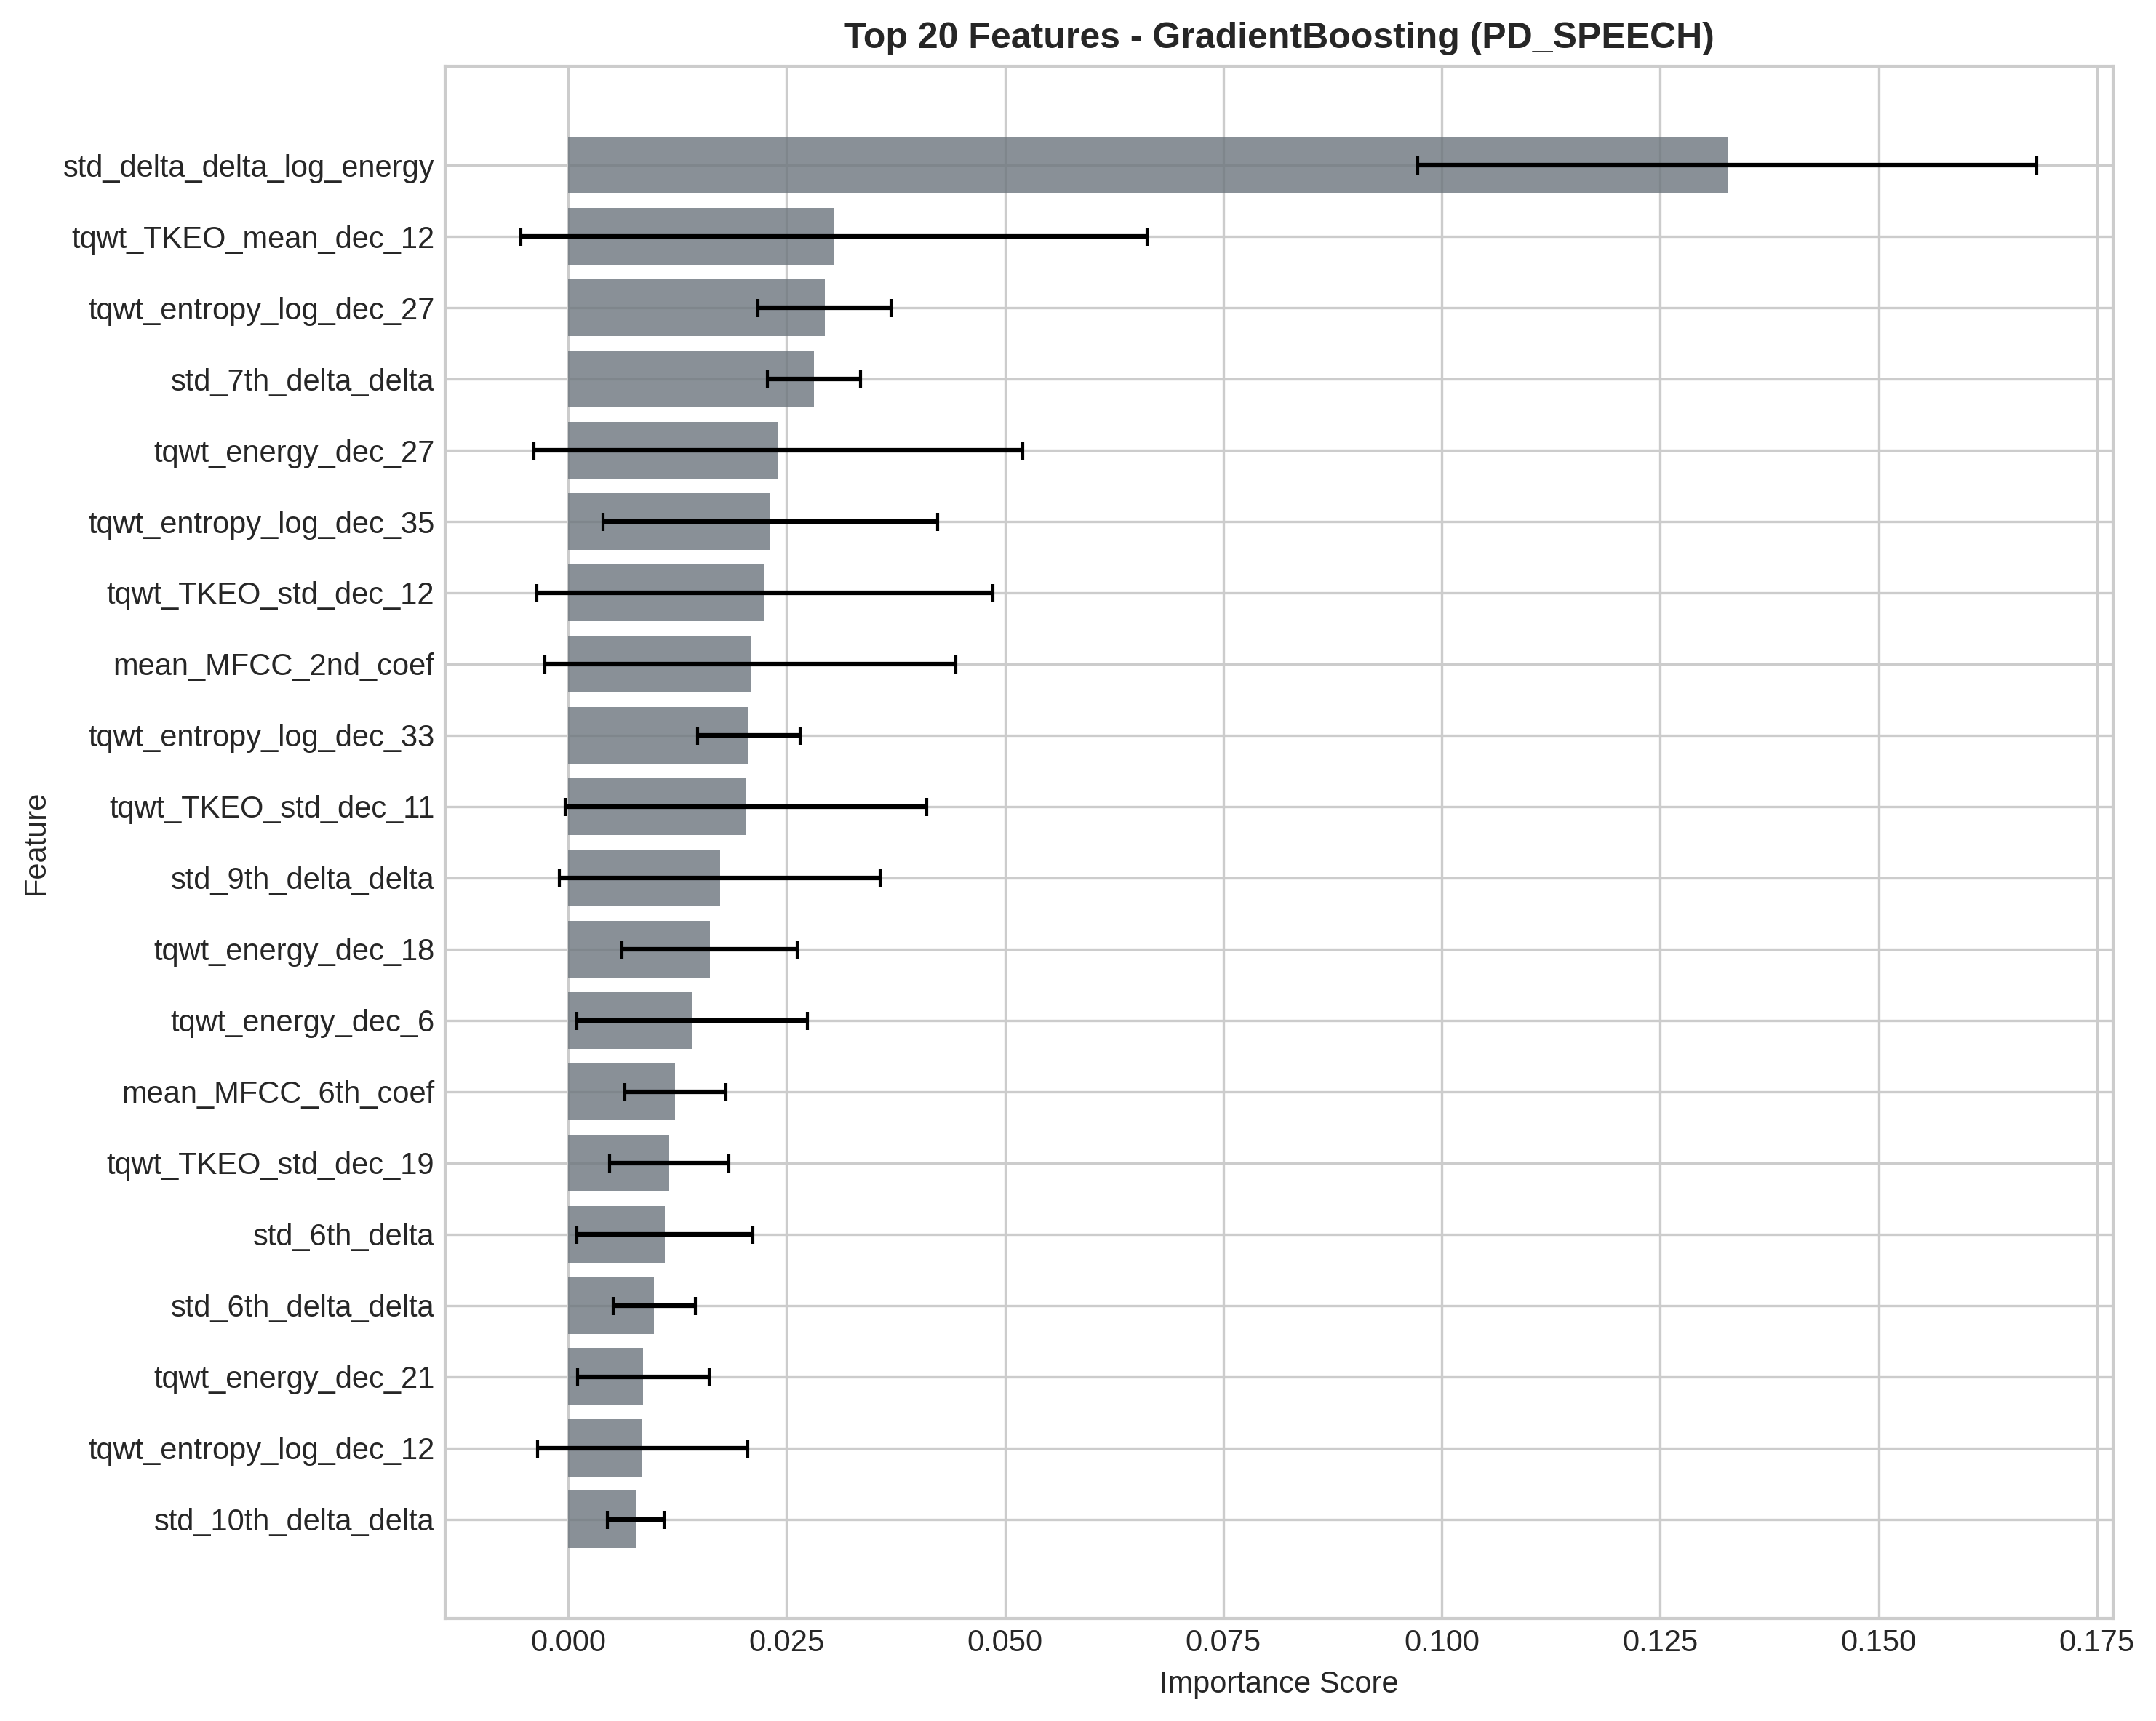
\includegraphics[width=\textwidth]{fig_imp_datasetb_gb.png}
        \caption{Gradient Boosting}
        \label{fig:imp-datasetb-gb}
    \end{subfigure}
    \hfill
    \begin{subfigure}[b]{0.48\textwidth}
        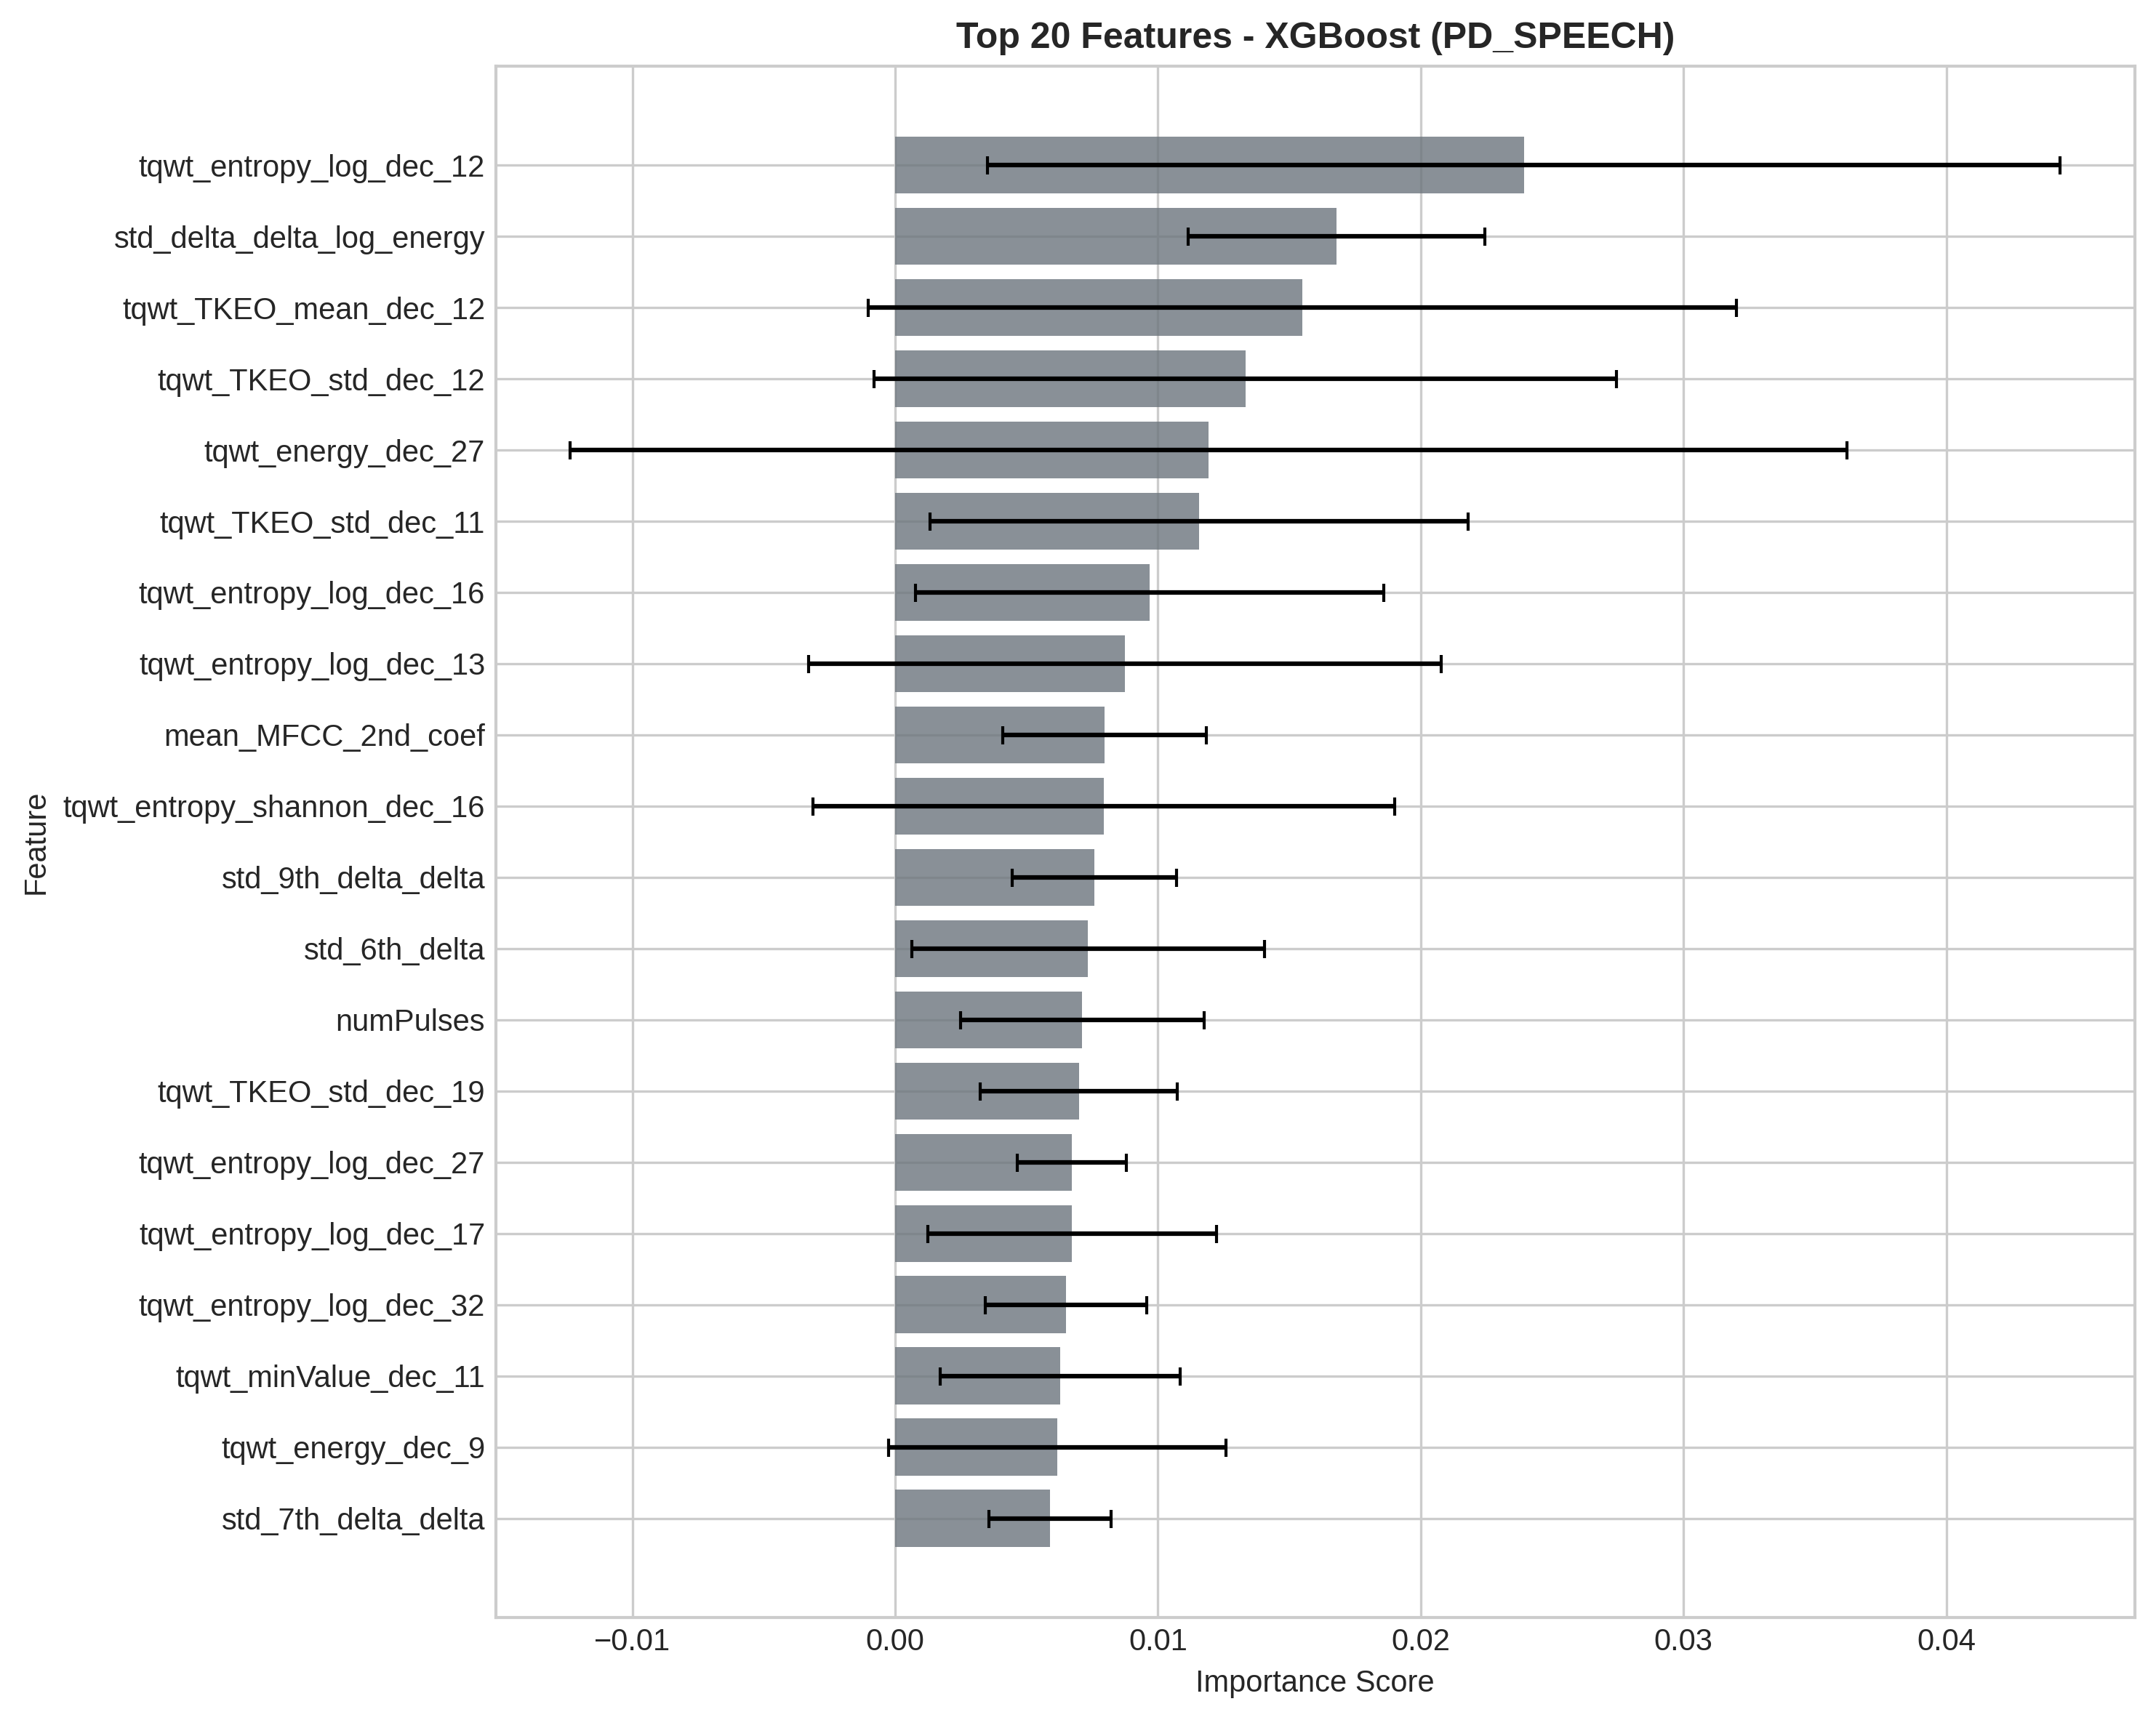
\includegraphics[width=\textwidth]{fig_imp_datasetb_xgb.png}
        \caption{XGBoost}
        \label{fig:imp-datasetb-xgb}
    \end{subfigure}
    \caption{Feature importance for Dataset B --- Gradient Boosting and XGBoost. TQWT energy/entropy features from high-frequency bands dominate across both models.}
    \label{fig:imp-datasetb-gb-xgb}
\end{figure}

\section{Cross-Task Feature Stability}

Features that appear in top-10 for both tasks (Random Forest) indicate robust discriminative power across different speech contexts:

\begin{table}[H]
\centering
\begin{tabular}{@{}lcc@{}}
\toprule
\textbf{Feature} & \textbf{ReadText Rank} & \textbf{Spontaneous Rank} \\
\midrule
delta\_mfcc\_2\_mean & 2 & 5 \\
autocorr\_harmonicity & 4 & 6 \\
f0\_mean & 6 & 10 \\
shimmer (apq3/apq11) & 7 & 2 \\
mfcc\_5\_mean & -- & 1 \\
f0\_std & -- & 9 \\
\bottomrule
\end{tabular}
\caption{Cross-task feature stability (Random Forest top-10)}
\label{tab:cross-task-features}
\end{table}

\textbf{Interpretation:} Features consistently important across tasks (delta\_mfcc\_2\_mean, autocorr\_harmonicity, shimmer) likely capture \textbf{task-general} acoustic signatures of PD rather than task-specific artifacts. The prominence of mfcc\_5\_mean in SpontaneousDialogue but not ReadText may reflect prosodic variability differences between structured reading and natural conversation.

\section{Feature Category Analysis}

Aggregating importance by feature category:

\begin{table}[H]
\centering
\begin{tabular}{@{}lccc@{}}
\toprule
\textbf{Category} & \textbf{Features} & \textbf{ReadText (\%)} & \textbf{Spontaneous (\%)} \\
\midrule
MFCC & 13 & 28.4 & 32.1 \\
Delta MFCC & 13 & 22.7 & 25.3 \\
Pitch ($F_0$) & 4 & 15.2 & 12.8 \\
Shimmer & 5 & 11.3 & 14.6 \\
Formants & 6 & 9.8 & 7.2 \\
Harmonicity & 2 & 6.1 & 4.3 \\
Other & 5 & 6.5 & 3.7 \\
\bottomrule
\end{tabular}
\caption{Aggregated feature importance by category}
\label{tab:category-importance}
\end{table}

\begin{figure}[H]
    \centering
    \begin{subfigure}[b]{0.48\textwidth}
        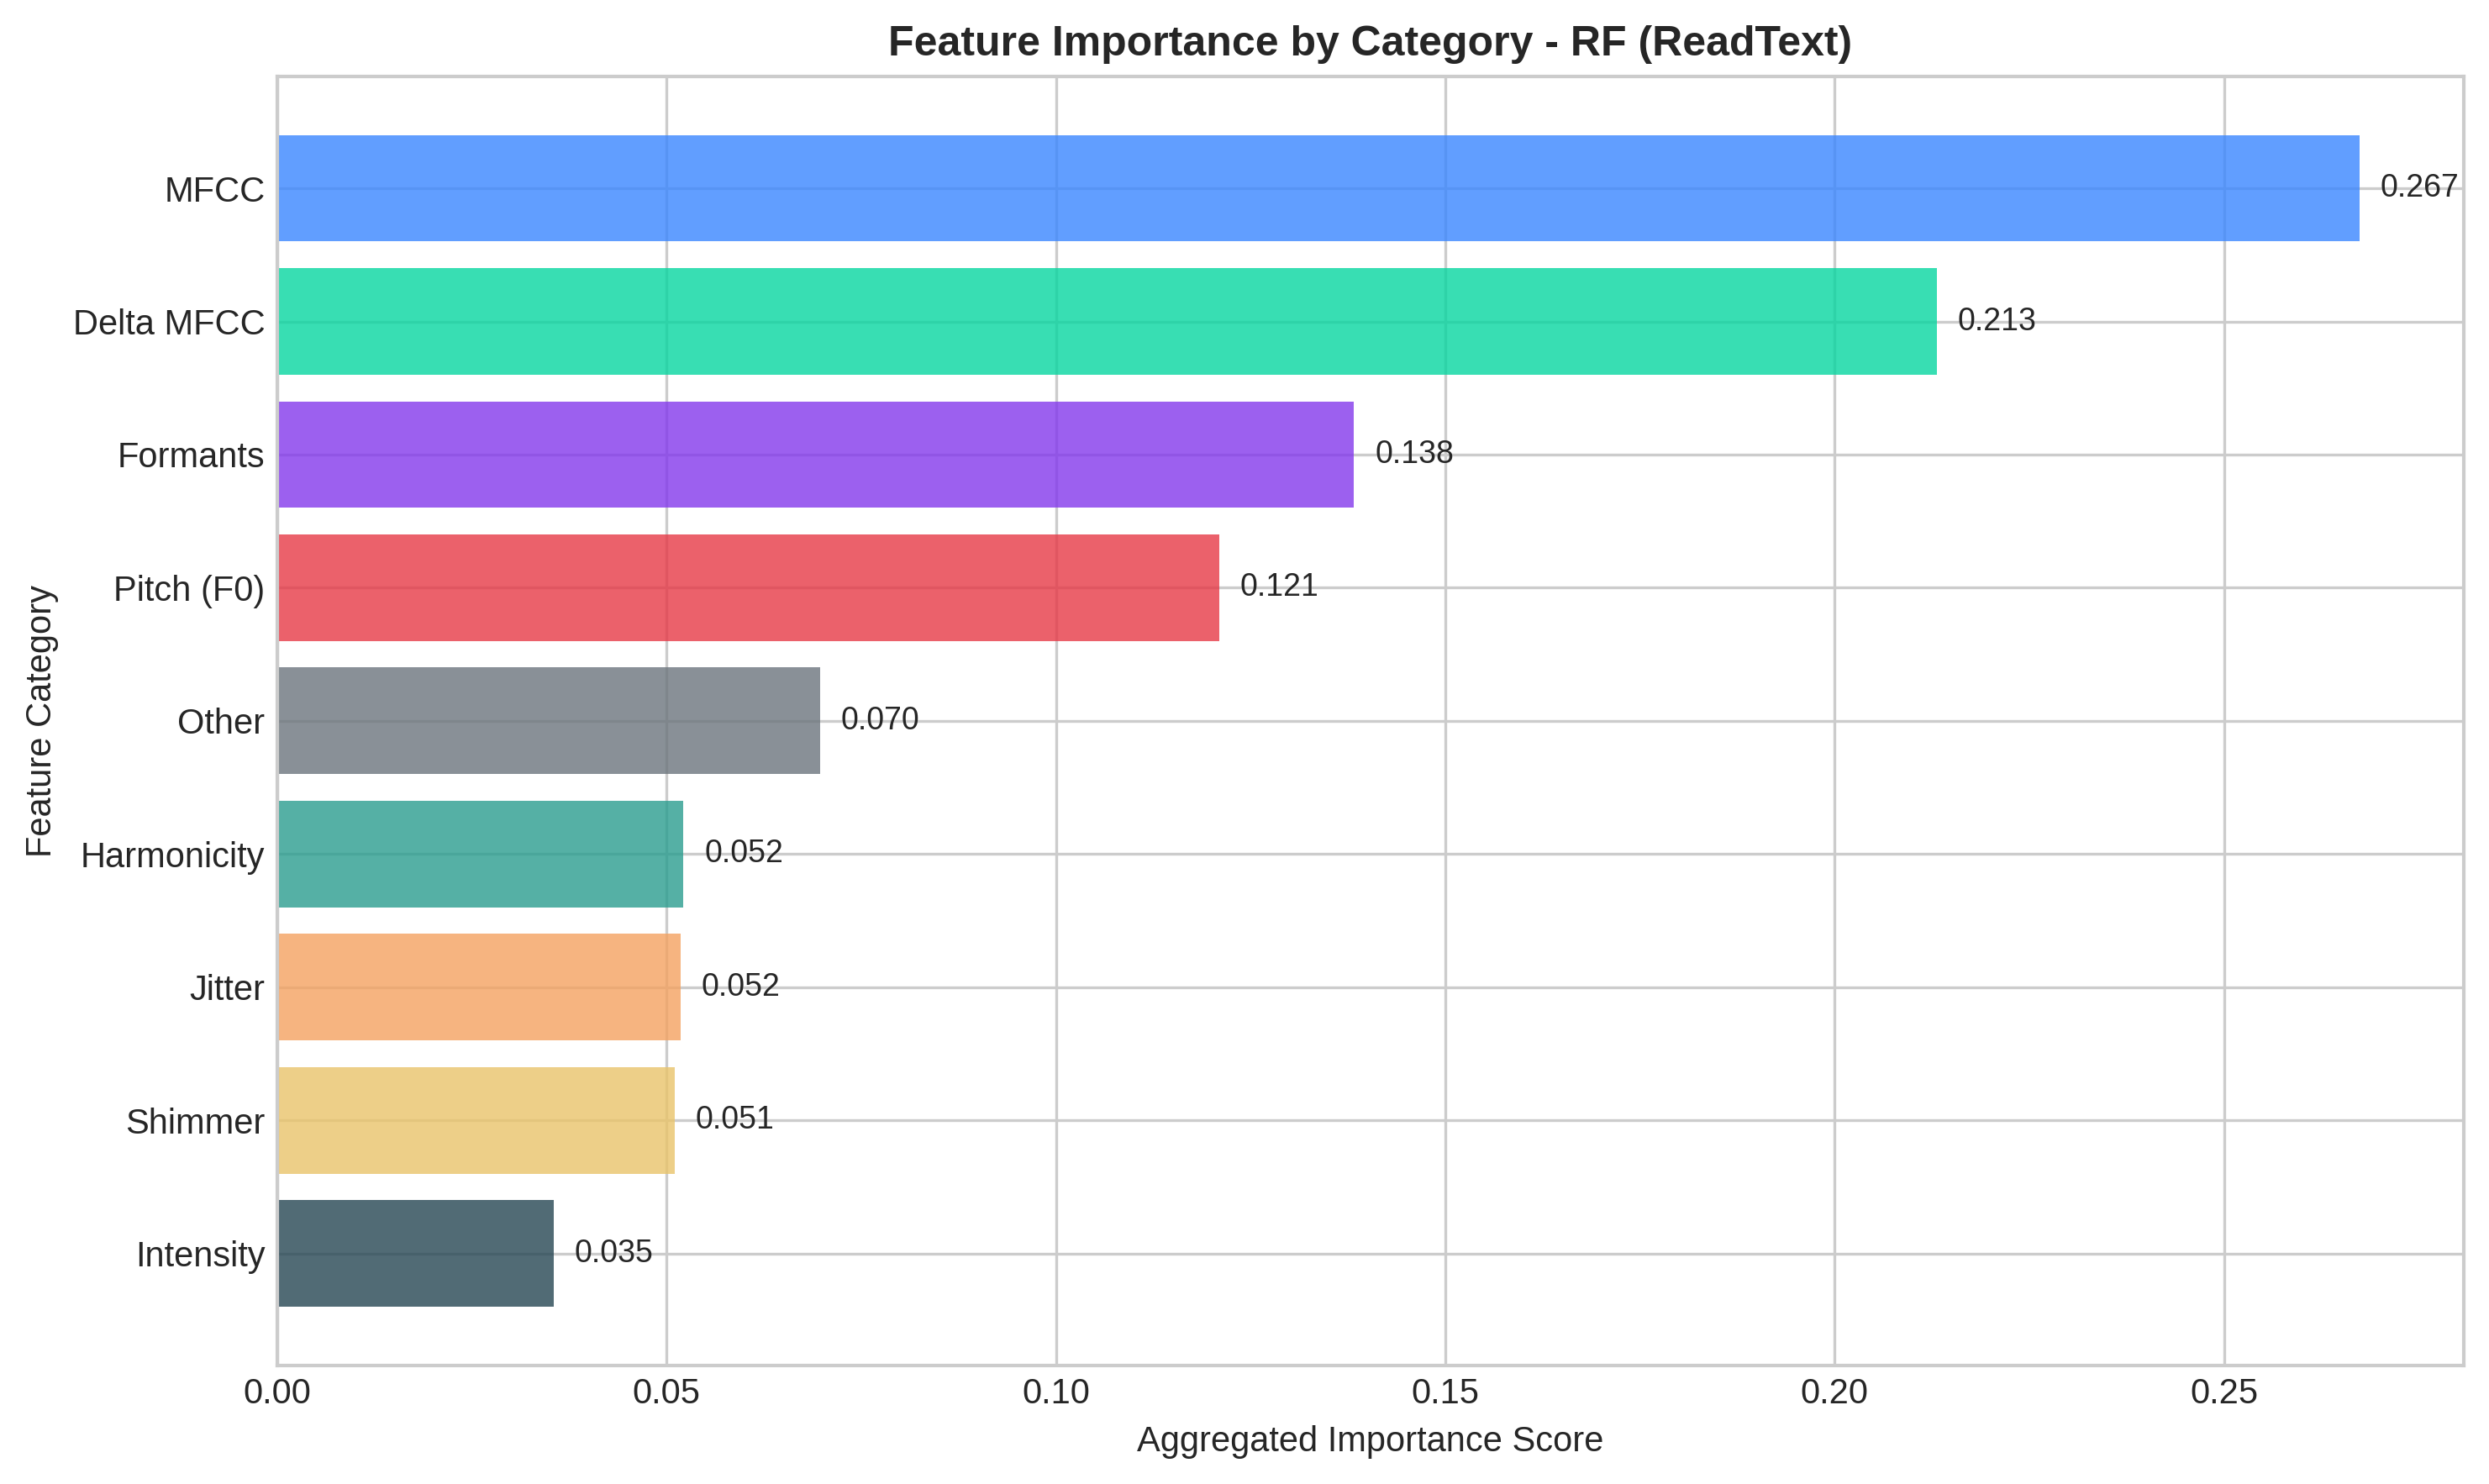
\includegraphics[width=\textwidth]{figures/fig_imp_readtext_cats.png}
        \caption{ReadText}
        \label{fig:imp-readtext-cats}
    \end{subfigure}
    \hfill
    \begin{subfigure}[b]{0.48\textwidth}
        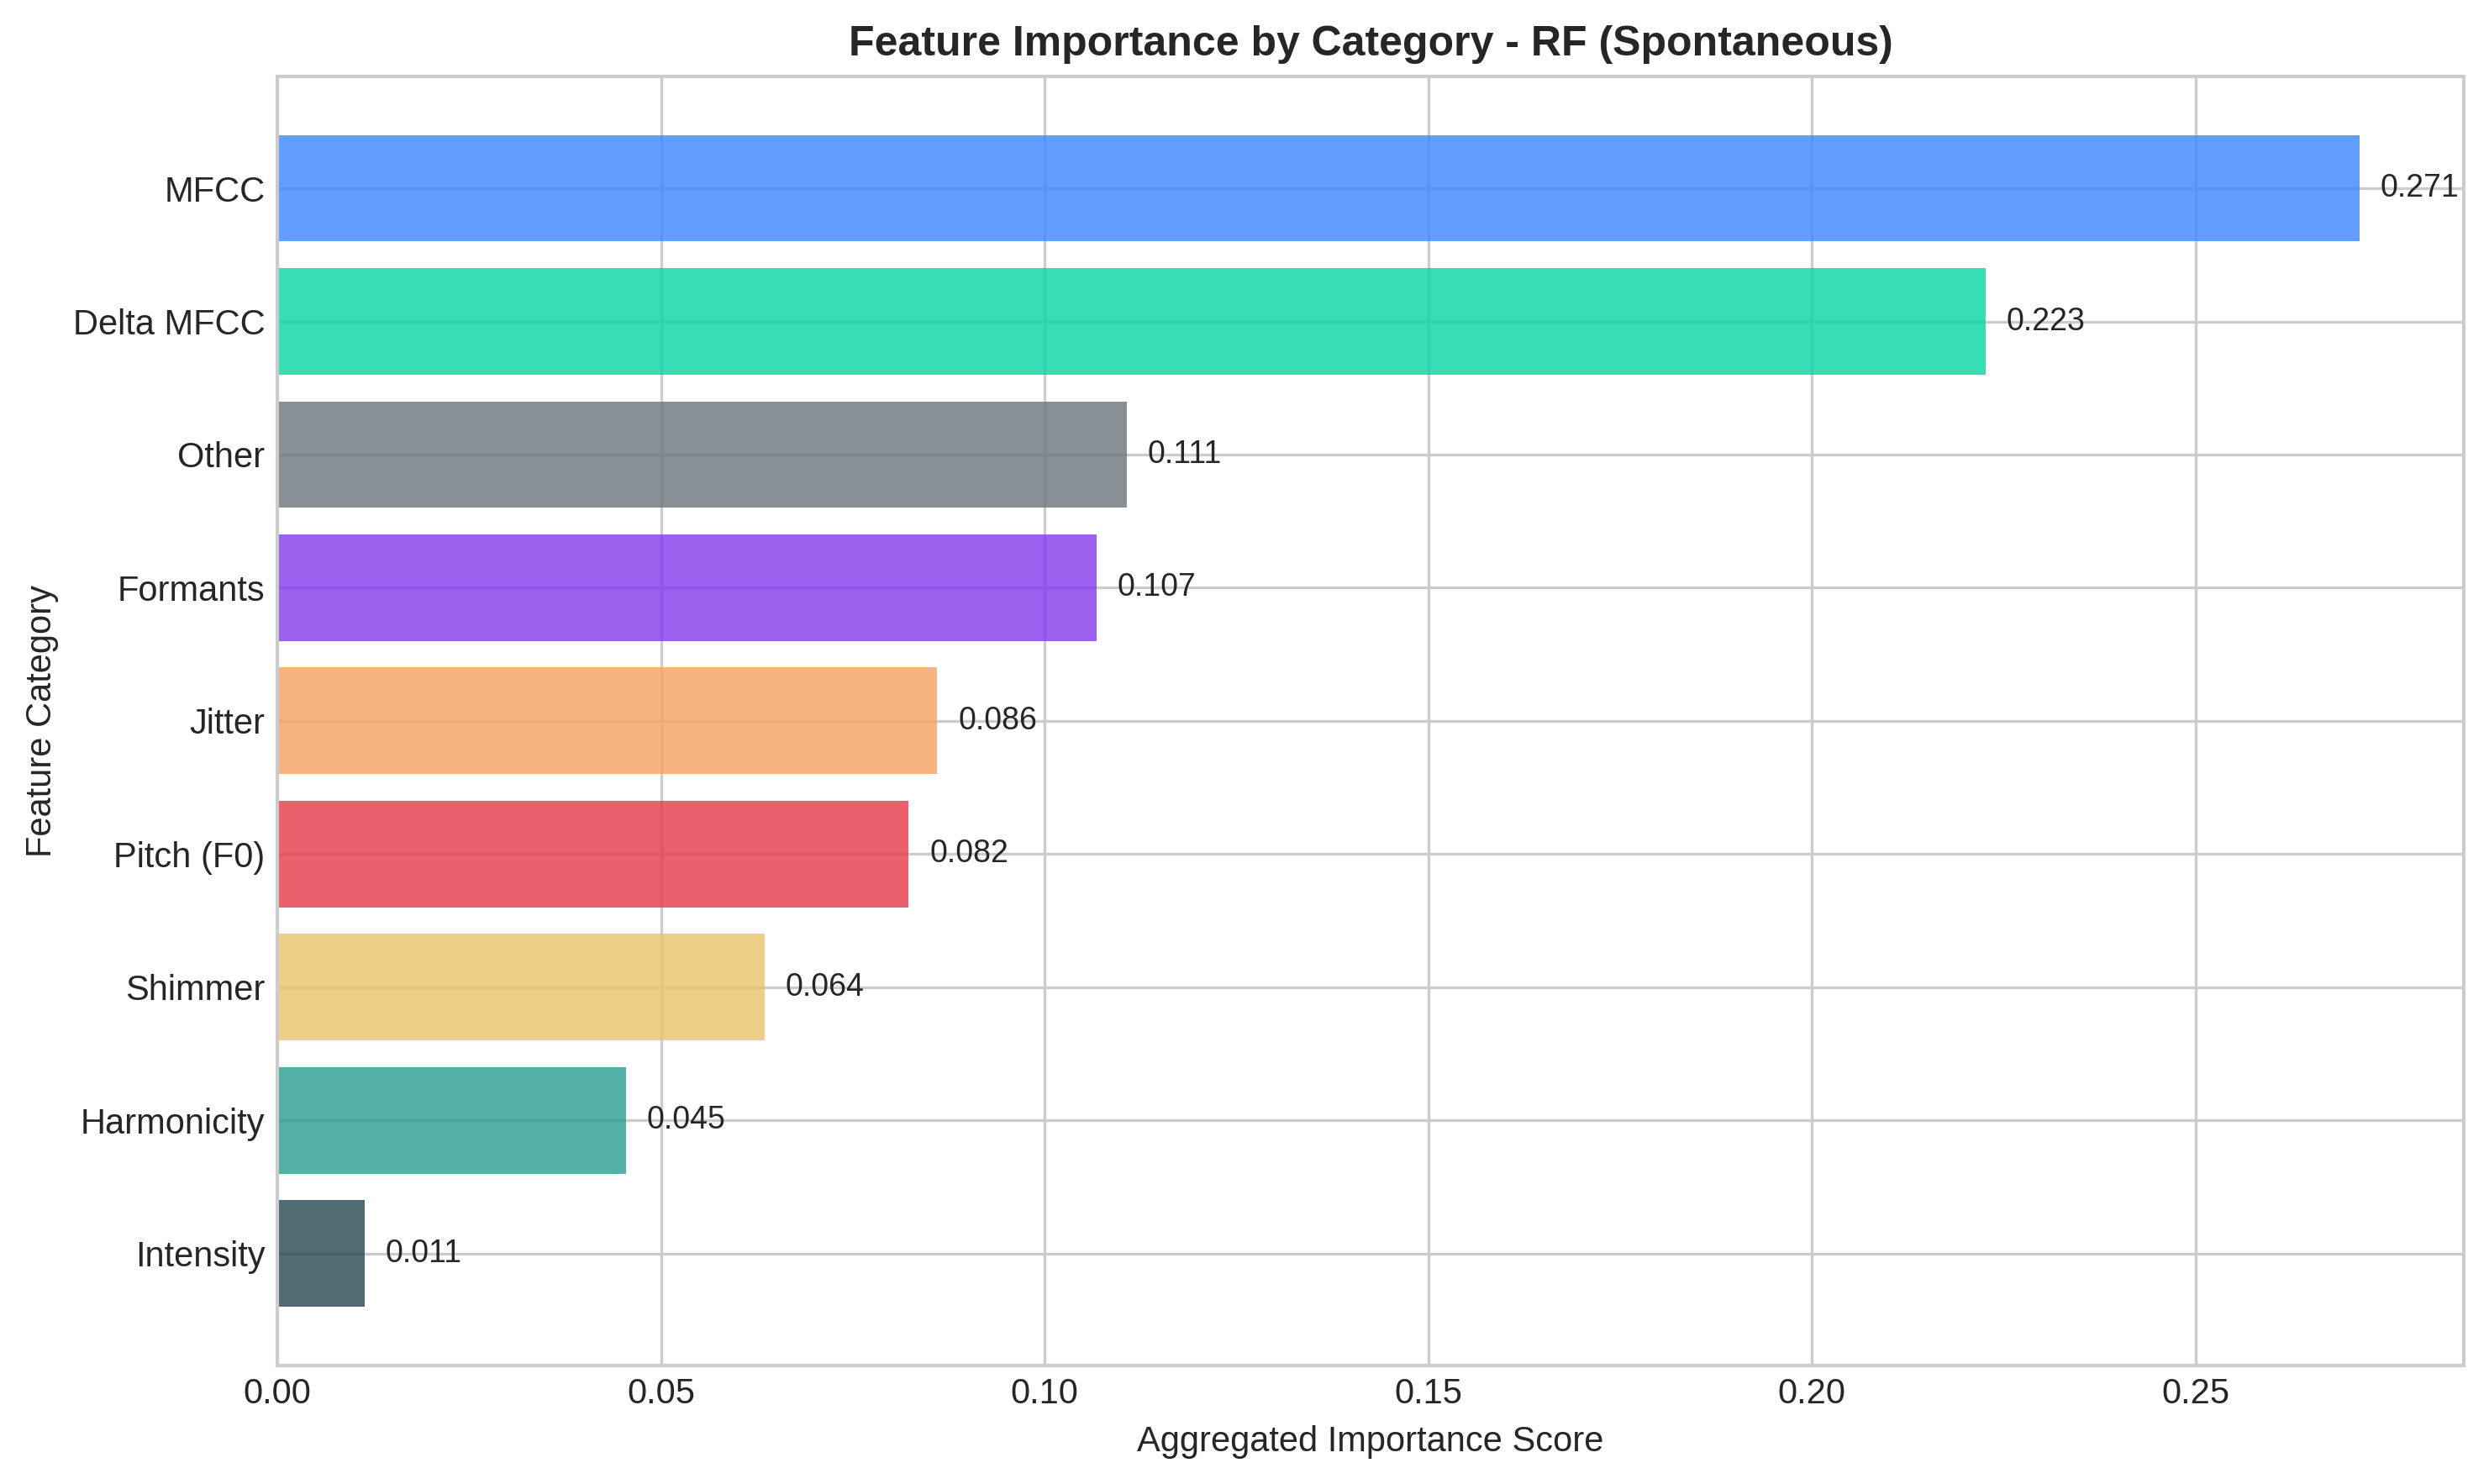
\includegraphics[width=\textwidth]{figures/fig_imp_spontaneous_cats.png}
        \caption{Spontaneous}
        \label{fig:imp-spontaneous-cats}
    \end{subfigure}
    \caption{Feature importance aggregated by broad acoustic categories.}
    \label{fig:imp-categories}
\end{figure}
}{}
\IfFileExists{appendices/appendix_b_results.tex}{% Παράρτημα B: Αναλυτικοί Πίνακες Αποτελεσμάτων

\chapter{Αναλυτικοί Πίνακες Αποτελεσμάτων}
\label{app:detailed-results}

\section{Επισκόπηση}

Το παρόν παράρτημα παρουσιάζει πλήρη αριθμητικά αποτελέσματα για όλες τις πειραματικές συνθήκες, συμπεριλαμβανομένων συνοπτικών στατιστικών και συγκρίσεων μεταξύ συνθηκών.

\section{Συνθήκη 1: Baseline Features (47) + Unweighted}
% Τα αποτελέσματα παράχθηκαν από το experimental pipeline (βλ. Chapter~\ref{ch:experimental-design})

\subsection{Dataset A: MDVR-KCL Σύνοψη}

\begin{table}[H]
\centering
\small
\begin{tabular}{@{}llccccc@{}}
\toprule
\textbf{Task} & \textbf{Model} & \textbf{Accuracy} & \textbf{Precision} & \textbf{Recall} & \textbf{F1} & \textbf{ROC-AUC} \\
\midrule
\multirow{3}{*}{ReadText} 
& LR & $0.621 \pm 0.058$ & $0.620 \pm 0.217$ & $0.550 \pm 0.201$ & $0.542 \pm 0.099$ & $0.717 \pm 0.139$ \\
& SVM & $0.621 \pm 0.106$ & $0.367 \pm 0.342$ & $0.317 \pm 0.335$ & $0.333 \pm 0.333$ & $0.614 \pm 0.312$ \\
& RF & $0.629 \pm 0.178$ & $0.450 \pm 0.447$ & $0.333 \pm 0.408$ & $0.351 \pm 0.363$ & $0.590 \pm 0.302$ \\
\midrule
\multirow{3}{*}{Spontaneous}
& LR & $0.639 \pm 0.160$ & $0.469 \pm 0.292$ & $0.667 \pm 0.408$ & $0.539 \pm 0.321$ & $0.760 \pm 0.214$ \\
& SVM & $0.636 \pm 0.135$ & $0.600 \pm 0.435$ & $0.333 \pm 0.236$ & $0.400 \pm 0.253$ & $0.407 \pm 0.309$ \\
& RF & $0.721 \pm 0.176$ & $0.633 \pm 0.415$ & $0.600 \pm 0.435$ & $0.567 \pm 0.365$ & $\mathbf{0.828 \pm 0.148}$ \\
\bottomrule
\end{tabular}
\caption{Αποτελέσματα Condition 1 ανά task (Dataset A, baseline features, χωρίς weighting)}
\label{tab:c1-summary}
\end{table}

\subsection{Dataset B: PD Speech Features Σύνοψη}

\begin{table}[H]
\centering
\small
\begin{tabular}{@{}lccccc@{}}
\toprule
\textbf{Model} & \textbf{Accuracy} & \textbf{Precision} & \textbf{Recall} & \textbf{F1} & \textbf{ROC-AUC} \\
\midrule
LogisticRegression & $0.828 \pm 0.008$ & $0.881 \pm 0.010$ & $0.890 \pm 0.016$ & $0.885 \pm 0.006$ & $0.867 \pm 0.029$ \\
SVM\_RBF & $0.851 \pm 0.024$ & $0.841 \pm 0.015$ & $0.986 \pm 0.019$ & $0.908 \pm 0.015$ & $0.885 \pm 0.025$ \\
RandomForest & $0.882 \pm 0.019$ & $0.876 \pm 0.012$ & $0.980 \pm 0.015$ & $0.925 \pm 0.012$ & $\mathbf{0.940 \pm 0.013}$ \\
\bottomrule
\end{tabular}
\caption{Αποτελέσματα Condition 1 (Dataset B, baseline features, χωρίς weighting)}
\label{tab:c1-datasetb}
\end{table}

\textbf{Σημείωση:} Το Dataset B εμφανίζει ουσιαστικά υψηλότερη απόδοση και χαμηλότερη διακύμανση από το Dataset A, εύρημα συμβατό με πιθανό optimistic bias λόγω άγνωστης επικάλυψης subjects.

\section{Συνθήκη 2: Extended Features (78) + Unweighted}
% Τα αποτελέσματα παράχθηκαν από το experimental pipeline (βλ. Chapter~\ref{ch:experimental-design})

\subsection{Dataset A: MDVR-KCL Σύνοψη}

\begin{table}[H]
\centering
\small
\begin{tabular}{@{}llccccc@{}}
\toprule
\textbf{Task} & \textbf{Model} & \textbf{Accuracy} & \textbf{Precision} & \textbf{Recall} & \textbf{F1} & \textbf{ROC-AUC} \\
\midrule
\multirow{3}{*}{ReadText} 
& LR & $0.596 \pm 0.079$ & $0.600 \pm 0.253$ & $0.433 \pm 0.149$ & $0.475 \pm 0.106$ & $0.698 \pm 0.132$ \\
& SVM & $0.786 \pm 0.181$ & $0.733 \pm 0.435$ & $0.567 \pm 0.365$ & $0.634 \pm 0.386$ & $0.834 \pm 0.153$ \\
& RF & $0.818 \pm 0.140$ & $0.883 \pm 0.162$ & $0.700 \pm 0.298$ & $0.746 \pm 0.207$ & $\mathbf{0.822 \pm 0.166}$ \\
\midrule
\multirow{3}{*}{Spontaneous}
& LR & $0.671 \pm 0.199$ & $0.500 \pm 0.361$ & $0.600 \pm 0.435$ & $0.530 \pm 0.377$ & $0.783 \pm 0.139$ \\
& SVM & $0.636 \pm 0.089$ & $0.533 \pm 0.361$ & $0.400 \pm 0.279$ & $0.428 \pm 0.258$ & $0.460 \pm 0.294$ \\
& RF & $0.779 \pm 0.161$ & $0.683 \pm 0.410$ & $0.600 \pm 0.435$ & $0.605 \pm 0.387$ & $\mathbf{0.857 \pm 0.171}$ \\
\bottomrule
\end{tabular}
\caption{Αποτελέσματα Condition 2 ανά task (Dataset A, extended features, χωρίς weighting)}
\label{tab:c2-summary}
\end{table}

\subsection{Βελτίωση έναντι Baseline (Random Forest, Dataset A)}

\begin{table}[H]
\centering
\begin{tabular}{@{}lccc@{}}
\toprule
\textbf{Task} & \textbf{$\Delta$ Accuracy} & \textbf{$\Delta$ ROC-AUC} & \textbf{$\Delta$ Variance} \\
\midrule
ReadText & +18.9pp & \textbf{+23.2pp} & Reduced (0.302 $\rightarrow$ 0.166) \\
SpontaneousDialogue & +5.8pp & +2.9pp & Increased (0.148 $\rightarrow$ 0.171) \\
\bottomrule
\end{tabular}
\caption{Βελτίωση Condition 2 έναντι Condition 1 (Random Forest)}
\label{tab:c2-improvement}
\end{table}

\textbf{Παρατήρηση:} Το feature extension βελτίωσε αισθητά την απόδοση στο ReadText (+23.2pp ROC-AUC), ενώ στο SpontaneousDialogue παρατηρήθηκαν πιο περιορισμένα gains (+2.9pp). Αυτό υποδηλώνει ότι τα extended features αποτυπώνουν αποτελεσματικότερα τις δυναμικές της δομημένης ομιλίας σε σύγκριση με την αυθόρμητη ομιλία.

\section{Συνθήκη 3: Baseline Features (47) + Weighted}
% Τα αποτελέσματα παράχθηκαν από το experimental pipeline (βλ. Chapter~\ref{ch:experimental-design})

\subsection{Dataset A: MDVR-KCL Σύνοψη}

\begin{table}[H]
\centering
\small
\begin{tabular}{@{}llccccc@{}}
\toprule
\textbf{Task} & \textbf{Model} & \textbf{Accuracy} & \textbf{Precision} & \textbf{Recall} & \textbf{F1} & \textbf{ROC-AUC} \\
\midrule
\multirow{3}{*}{ReadText} 
& LR & $0.596 \pm 0.079$ & $0.600 \pm 0.235$ & $0.550 \pm 0.201$ & $0.528 \pm 0.099$ & $0.717 \pm 0.139$ \\
& SVM & $0.704 \pm 0.111$ & $0.617 \pm 0.371$ & $0.500 \pm 0.373$ & $0.519 \pm 0.320$ & $0.542 \pm 0.312$ \\
& RF & $0.650 \pm 0.148$ & $0.550 \pm 0.371$ & $0.400 \pm 0.365$ & $0.431 \pm 0.306$ & $0.687 \pm 0.258$ \\
\midrule
\multirow{3}{*}{Spontaneous}
& LR & $0.639 \pm 0.160$ & $0.469 \pm 0.292$ & $0.667 \pm 0.408$ & $0.539 \pm 0.321$ & $0.760 \pm 0.214$ \\
& SVM & $0.693 \pm 0.123$ & $0.567 \pm 0.365$ & $0.600 \pm 0.365$ & $0.560 \pm 0.318$ & $0.423 \pm 0.312$ \\
& RF & $0.693 \pm 0.123$ & $0.583 \pm 0.373$ & $0.600 \pm 0.435$ & $0.538 \pm 0.326$ & $\mathbf{0.827 \pm 0.133}$ \\
\bottomrule
\end{tabular}
\caption{Αποτελέσματα Condition 3 ανά task (Dataset A, baseline features, με weighting)}
\label{tab:c3-summary}
\end{table}

\subsection{Επίδραση του Weighting (vs Condition 1, Random Forest)}

\begin{table}[H]
\centering
\begin{tabular}{@{}lccc@{}}
\toprule
\textbf{Task} & \textbf{$\Delta$ Accuracy} & \textbf{$\Delta$ ROC-AUC} & \textbf{Effect} \\
\midrule
ReadText & +2.1pp & +9.7pp & Improved \\
SpontaneousDialogue & $-2.8$pp & $-0.1$pp & Negligible \\
\bottomrule
\end{tabular}
\caption{Επίδραση του weighting στο Condition 3 έναντι Condition 1 (RF)}
\label{tab:c3-weighting}
\end{table}

\textbf{Παρατήρηση:} Το class weighting βελτίωσε την απόδοση στο ReadText, αλλά είχε αμελητέα επίδραση στο SpontaneousDialogue, γεγονός που υποδηλώνει task-dependent ευαισθησία στον χειρισμό του class imbalance.

\section{Συνθήκη 4: Extended Features (78) + Weighted}
% Τα αποτελέσματα παράχθηκαν από το experimental pipeline (βλ. Chapter~\ref{ch:experimental-design})

\subsection{Dataset A: MDVR-KCL Σύνοψη}

\begin{table}[H]
\centering
\small
\begin{tabular}{@{}llccccc@{}}
\toprule
\textbf{Task} & \textbf{Model} & \textbf{Accuracy} & \textbf{Precision} & \textbf{Recall} & \textbf{F1} & \textbf{ROC-AUC} \\
\midrule
\multirow{3}{*}{ReadText} 
& LR & $0.650 \pm 0.108$ & $0.650 \pm 0.253$ & $0.550 \pm 0.201$ & $0.564 \pm 0.160$ & $0.698 \pm 0.132$ \\
& SVM & $0.761 \pm 0.214$ & $0.700 \pm 0.447$ & $0.567 \pm 0.365$ & $0.620 \pm 0.390$ & $0.834 \pm 0.153$ \\
& RF & $0.818 \pm 0.140$ & $0.883 \pm 0.162$ & $0.700 \pm 0.298$ & $0.746 \pm 0.207$ & $0.805 \pm 0.182$ \\
\midrule
\multirow{3}{*}{Spontaneous}
& LR & $0.696 \pm 0.179$ & $0.520 \pm 0.356$ & $0.667 \pm 0.471$ & $0.563 \pm 0.381$ & $0.783 \pm 0.139$ \\
& SVM & $0.664 \pm 0.167$ & $0.567 \pm 0.365$ & $0.600 \pm 0.365$ & $0.560 \pm 0.318$ & $0.403 \pm 0.347$ \\
& RF & $0.721 \pm 0.203$ & $0.653 \pm 0.409$ & $0.600 \pm 0.435$ & $0.583 \pm 0.373$ & $\mathbf{0.823 \pm 0.209}$ \\
\bottomrule
\end{tabular}
\caption{Αποτελέσματα Condition 4 ανά task (Dataset A, extended features, με weighting)}
\label{tab:c4-summary}
\end{table}

\subsection{Επίδραση του Weighting (vs Condition 2, Random Forest)}

\begin{table}[H]
\centering
\begin{tabular}{@{}lccc@{}}
\toprule
\textbf{Task} & \textbf{$\Delta$ Accuracy} & \textbf{$\Delta$ ROC-AUC} & \textbf{Effect} \\
\midrule
ReadText & 0.0pp & $-1.7$pp & Slight decrease \\
SpontaneousDialogue & $-5.8$pp & $-3.4$pp & Decreased \\
\bottomrule
\end{tabular}
\caption{Επίδραση του weighting στο Condition 4 έναντι Condition 2 (RF)}
\label{tab:c4-weighting}
\end{table}

\textbf{Παρατήρηση:} Ο συνδυασμός extended features με class weighting δεν βελτίωσε την απόδοση σε σχέση με τη χρήση extended features μόνο. Αυτό υποδηλώνει ότι feature extension και class weighting αντιμετωπίζουν παρόμοιες πτυχές του classification problem, με diminishing returns όταν εφαρμόζονται από κοινού.

\section{Matrix Σύγκρισης μεταξύ Conditions}

\subsection{Random Forest ROC-AUC ανά Task}

\begin{table}[H]
\centering
\begin{tabular}{@{}llcc@{}}
\toprule
\textbf{Task} & & \textbf{Baseline (47)} & \textbf{Extended (78)} \\
\midrule
\multirow{2}{*}{ReadText}
& Unweighted & $0.590 \pm 0.302$ & $\mathbf{0.822 \pm 0.166}$ \\
& Weighted & $0.687 \pm 0.258$ & $0.805 \pm 0.182$ \\
\midrule
\multirow{2}{*}{Spontaneous}
& Unweighted & $0.828 \pm 0.148$ & $\mathbf{0.857 \pm 0.171}$ \\
& Weighted & $0.827 \pm 0.133$ & $0.823 \pm 0.209$ \\
\bottomrule
\end{tabular}
\caption{Πίνακας σύγκρισης Random Forest ROC-AUC (Dataset A)}
\label{tab:rf-rocauc-matrix}
\end{table}

\subsection{Random Forest Accuracy ανά Task}

\begin{table}[H]
\centering
\begin{tabular}{@{}llcc@{}}
\toprule
\textbf{Task} & & \textbf{Baseline (47)} & \textbf{Extended (78)} \\
\midrule
\multirow{2}{*}{ReadText}
& Unweighted & $62.9\% \pm 17.8\%$ & $\mathbf{81.8\% \pm 14.0\%}$ \\
& Weighted & $65.0\% \pm 14.8\%$ & $81.8\% \pm 14.0\%$ \\
\midrule
\multirow{2}{*}{Spontaneous}
& Unweighted & $72.1\% \pm 17.6\%$ & $\mathbf{77.9\% \pm 16.1\%}$ \\
& Weighted & $69.3\% \pm 12.3\%$ & $72.1\% \pm 20.3\%$ \\
\bottomrule
\end{tabular}
\caption{Πίνακας σύγκρισης Random Forest Accuracy (Dataset A)}
\label{tab:rf-accuracy-matrix}
\end{table}

\subsection{Κύριες Παρατηρήσεις}

\begin{enumerate}
    \item \textbf{Το feature extension βελτιώνει σταθερά το ReadText:} +23.2pp ROC-AUC (χωρίς weighting)
    \item \textbf{Το SpontaneousDialogue έχει υψηλότερο baseline:} 0.828 vs 0.590 ROC-AUC με baseline features
    \item \textbf{Το class weighting εμφανίζει μικτά αποτελέσματα:} βελτιώνει τη baseline επίδοση στο ReadText αλλά μειώνει την επίδοση με extended features
    \item \textbf{Υψηλή διακύμανση σε όλα τα settings:} τα standard deviations συχνά υπερβαίνουν το 0.15, αντανακλώντας το μικρό sample size ($n=37$)
\end{enumerate}

\section{Σημειώσεις για τη Statistical Significance}

Λόγω υψηλών standard deviations (συχνά $> 0.15$), τα confidence intervals επικαλύπτονται σε πολλές συγκρίσεις. Αυτό περιορίζει τη δυνατότητα για ισχυρούς στατιστικούς ισχυρισμούς σχετικά με τις διαφορές μεταξύ conditions. Τα αποτελέσματα θα πρέπει να ερμηνεύονται ως \textbf{trends} και όχι ως οριστικές κατατάξεις.

\section{Καμπύλες ROC}

Παρουσιάζονται καμπύλες Receiver Operating Characteristic (ROC) για όλους τους πέντε classifiers σε κάθε experimental condition. Οι αχνές καμπύλες αντιστοιχούν σε μεμονωμένα cross-validation folds, ενώ η έντονη καμπύλη αντιστοιχεί στον μέσο όρο των folds με shaded band $\pm 1$ standard deviation. Όλες οι καμπύλες δημιουργήθηκαν με χρήση του extended feature set.

\begin{figure}[H]
    \centering
    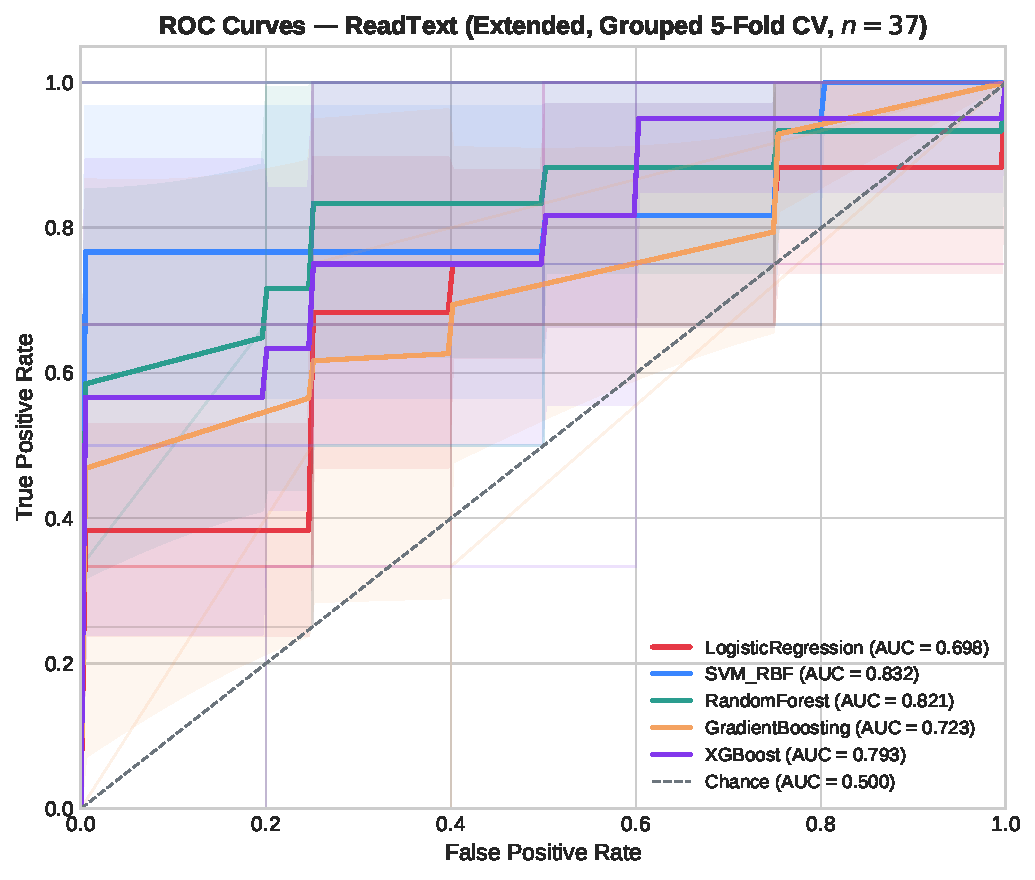
\includegraphics[width=\textwidth]{fig_roc_readtext.pdf}
    \caption{ROC curves για όλους τους πέντε classifiers στο ReadText task (Dataset A, extended features). Τα shaded bands υποδεικνύουν $\pm 1$ standard deviation στα πέντε cross-validation folds.}
    \label{fig:roc-readtext}
\end{figure}

\begin{figure}[H]
    \centering
    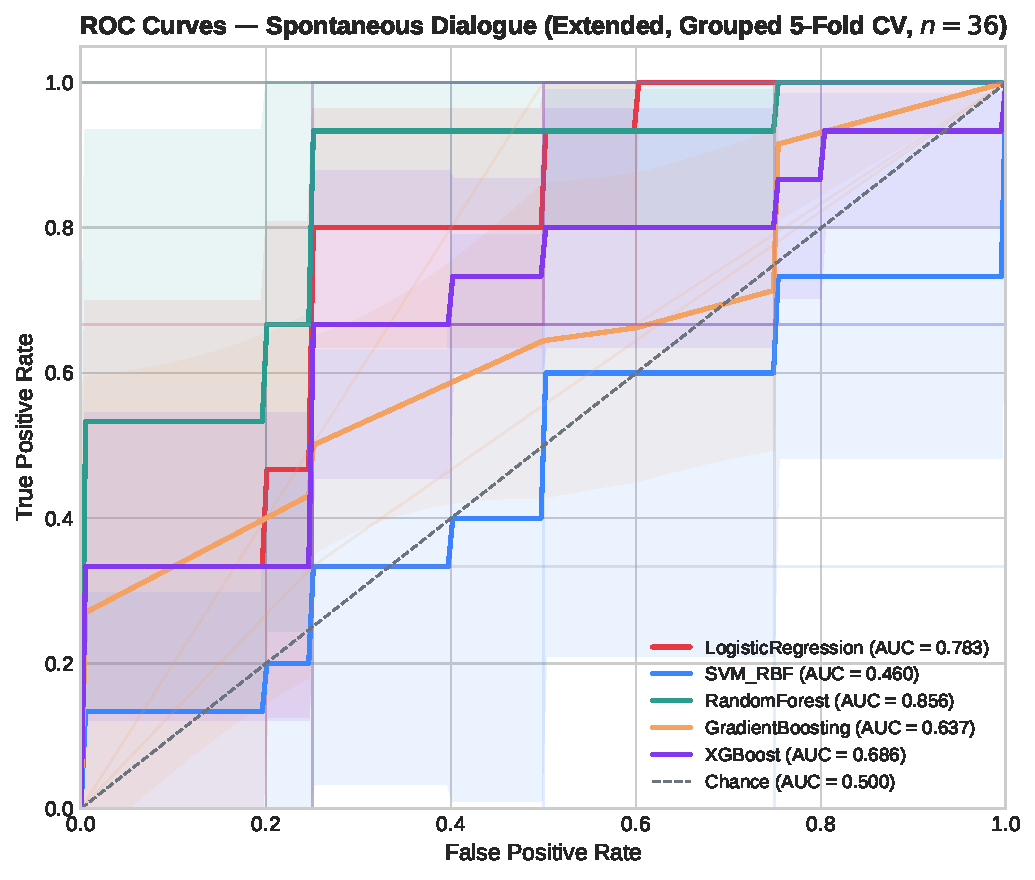
\includegraphics[width=\textwidth]{fig_roc_spontaneous.pdf}
    \caption{ROC curves για όλους τους πέντε classifiers στο SpontaneousDialogue task (Dataset A, extended features).}
    \label{fig:roc-spontaneous}
\end{figure}

\begin{figure}[H]
    \centering
    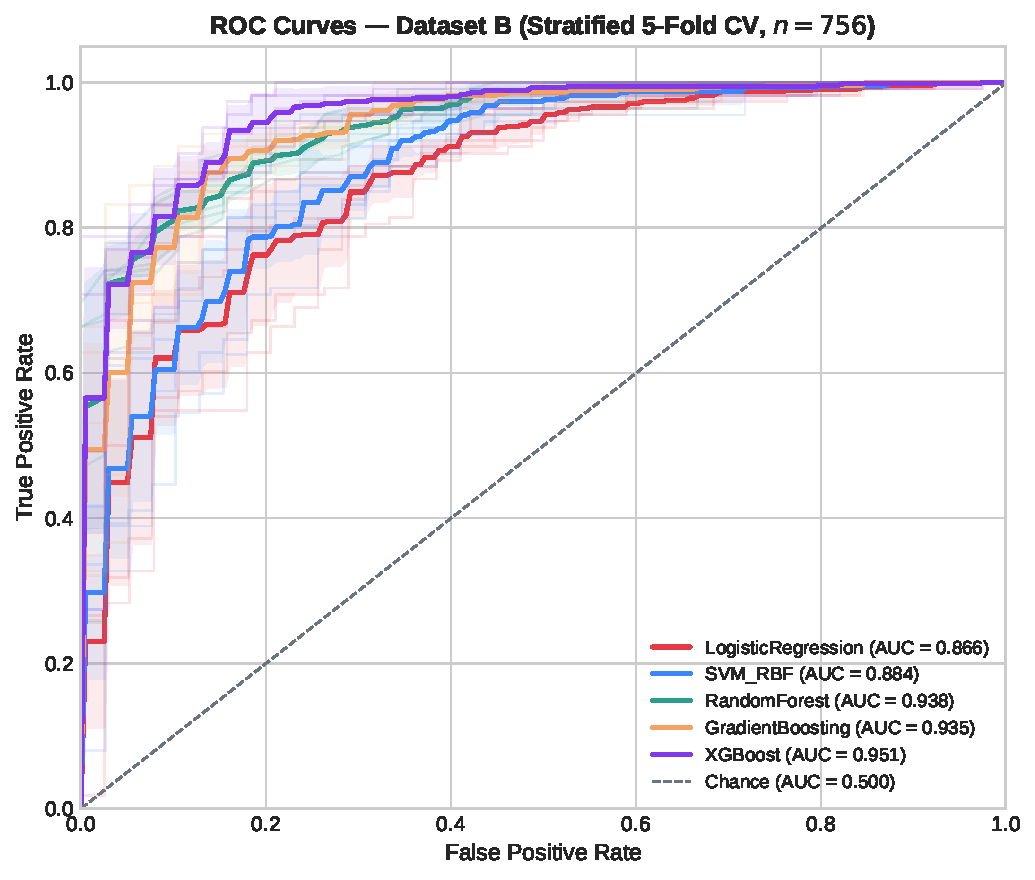
\includegraphics[width=\textwidth]{fig_roc_dataset_b.pdf}
    \caption{ROC curves για όλους τους πέντε classifiers στο Dataset B (PD Speech Features). Σημειώνεται ότι subject-level deduplication δεν είναι εφικτό για αυτό το dataset· τα αποτελέσματα ενδέχεται να είναι optimistic λόγω πιθανής επικάλυψης subjects μεταξύ folds.}
    \label{fig:roc-datasetb}
\end{figure}
}{}

\end{document}
